\documentclass[openany]{stml-l}
\usepackage[ngerman]{babel}
\usepackage[utf8]{inputenc}
\usepackage[T1]{fontenc}
\usepackage{amsmath,amssymb}
\usepackage{amsthm}
\usepackage{graphicx}
\usepackage{caption}
\usepackage{subcaption}
\usepackage{empheq}
\usepackage{hyperref}
\usepackage{float}
\usepackage[backend=biber,style=authoryear]{biblatex}

\addbibresource{bibliography/literatur.bib}

\graphicspath{{images/}}

\newtheorem{theorem}{Theorem}
\newtheorem{definition}{Definition}[section]
\newtheorem{satz}[definition]{Satz}
\newtheorem{lemma}[definition]{Lemma}
\newtheorem{korollar}[definition]{Korollar}
\newtheorem{beispiel}[definition]{Beispiel}
\newtheorem{bemerkung}[definition]{Bemerkung}
\newtheorem{hilfssatz}[definition]{Hilfssatz}
\begin{document}
\begin{titlepage}
    \begin{center}
        \par\huge \textsc{Eliptische Kurven Kryptographie}
    \end{center}

    \medskip

    \begin{center}
        \textsc{Masterarbeit}

        \bigskip
        Autor:\\ %Use different gender if preferred.
        Philipp Eckstein, 3554663\\
        \smallskip
        Betreuer:\\ %Use different gender if preferred.
        Prof. Dr. Meinolf Geck\\
        \bigskip
        Universität Stuttgart\\
        Institut für Diskrete Strukturen und Symbolisches Rechnen
        \vfill

        \begin{figure}[ht]
            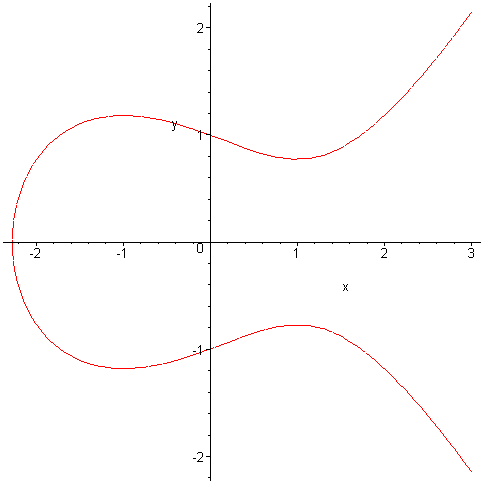
\includegraphics[width=0.5\textwidth]{ElliptischeKurven.png}
            \captionsetup{labelformat=empty} %surpresses enumeration
            \caption{Elliptische Kurve $\displaystyle 5y^{2}=x^{3}-3x+5$ über dem Körper der reellen Zahlen Quelle: \url{https://de.wikipedia.org/wiki/Elliptische_Kurve} }
        \end{figure}
    \end{center}
    \vfill
\end{titlepage}

\chapter{Vorwort}

\section*{Eidesstattliche Erklärung}
Hier sollte eine kluge Eidesstattliche Erklärung stehen, dass du alles allein gemacht hast et cetera et cetera.
\bigskip\underline{\hspace{0.2\textwidth}}\hspace{0.1\textwidth}\underline{\hspace{0.4\textwidth}}
\section*{Danksagung}
An erster Stelle dankt man meistens dem Betreuer. Je nach Sentimentalität kann dann auch weiteren Personen aus dem akademischen oder dem privaten Umfeld gedankt werden.
\section{Einführung}
(Grundlagen der Kryptographie, vgl. S.2ff.)
Der Wunsch, Informationen vor dem Zugriff unbefugter Personen zu schützen,
reicht weit in die Geschichte zurück. Bereits Julius Caesar soll ein
Verschlüsselungsverfahren verwendet haben, um militärische Nachrichten
vertraulich zu übermitteln. Bei der heute als Caesar-Chiffre bezeichneten
Methode werden die Buchstaben des Alphabets um eine festgelegte Anzahl von
Stellen verschoben. Nur wer die verwendete Verschiebung kennt, kann die
Nachricht unmittelbar entschlüsseln \cite[S.~14--15]{buell24}. Aus heutiger
Sicht bietet dieses Verfahren keine ausreichende Sicherheit, veranschaulicht
jedoch bereits ein grundlegendes Prinzip der Kryptographie: Eine Nachricht
wird mithilfe eines Schlüssels so verändert, dass ihr ursprünglicher Inhalt
für Unbefugte nicht mehr erkennbar ist.

Mit der zunehmenden Digitalisierung hat die sichere Übertragung von
Informationen erheblich an Bedeutung gewonnen. Beim Onlinebanking, bei der
E-Mail-Kommunikation und bei der Nutzung von Nachrichtendiensten werden
regelmäßig sensible Daten über öffentliche Netzwerke übertragen.
Kryptographische Verfahren sollen unter anderem gewährleisten, dass diese
Informationen nicht von unbefugten Dritten gelesen oder unbemerkt verändert
werden können.

Eine wichtige Rolle spielt dabei die asymmetrische Kryptographie, bei der
öffentliche und private Schlüssel verwendet werden. Die Sicherheit der
entsprechenden Verfahren beruht häufig auf mathematischen Problemen, für die
auf klassischen Computern keine effizienten Lösungsverfahren bekannt sind.
Zu diesen Problemen gehört das diskrete Logarithmusproblem. Wird es in der
Punktgruppe einer elliptischen Kurve über einem endlichen Körper betrachtet,
bildet es eine wesentliche Sicherheitsgrundlage der
Elliptische-Kurven-Kryptographie.

Die Entwicklung von Quantencomputern stellt diese Sicherheitsannahme
grundsätzlich infrage. Insbesondere ermöglicht der Shor-Algorithmus,
diskrete Logarithmusprobleme auf einem hinreichend leistungsfähigen
Quantencomputer effizient zu lösen. Daher ist zu untersuchen, welche
Konsequenzen sich aus der Entwicklung von Quantencomputern für die Sicherheit
kryptographischer Verfahren auf elliptischen Kurven ergeben.

\section{Zielsetzung und Forschungsfrage}

Ziel dieser Arbeit ist es, elliptische Kurven mathematisch einzuführen und
ihre Verwendung in der Kryptographie darzustellen. Dazu werden elliptische
Kurven über endlichen Körpern sowie das diskrete Logarithmusproblem in ihren
Punktgruppen untersucht. Anschließend werden die Grundlagen des
Quantencomputings und insbesondere der Shor-Algorithmus betrachtet, um dessen
Auswirkungen auf die Sicherheit der Elliptische-Kurven-Kryptographie zu
bewerten.

Daraus ergibt sich die folgende Forschungsfrage:

\begin{quote}
    \emph{Wie verändert der Shor-Algorithmus die Komplexität des diskreten
        Logarithmusproblems auf elliptischen Kurven, und welche Konsequenzen
        ergeben sich daraus für die Sicherheit der
        Elliptische-Kurven-Kryptographie?}
\end{quote}

\section{Aufbau der Arbeit}

Zunächst werden die für die weitere Untersuchung benötigten Grundlagen der
asymmetrischen Kryptographie eingeführt. Das RSA-Kryptosystem dient dabei als
Beispiel, um das Zusammenspiel öffentlicher und privater Schlüssel sowie das
Prinzip der asymmetrischen Verschlüsselung zu erläutern. Anschließend wird das
diskrete Logarithmusproblem zunächst in einer allgemeinen Gruppe formuliert.

Darauf folgt die mathematische Einführung elliptischer Kurven. Neben ihrer
Definition werden insbesondere die Gruppenstruktur, die Punktaddition und die
Skalarmultiplikation behandelt. Anschließend werden elliptische Kurven über
endlichen Körpern untersucht, da deren endliche Punktgruppen die Grundlage
kryptographischer Anwendungen bilden.

Auf diesen Grundlagen aufbauend wird das diskrete Logarithmusproblem auf
elliptischen Kurven betrachtet und seine Bedeutung für die Sicherheit
kryptographischer Verfahren erläutert. Danach werden ausgewählte
kryptographische Verfahren auf elliptischen Kurven vorgestellt.

Im letzten Teil der Arbeit werden zunächst die erforderlichen Grundlagen des
Quantencomputings eingeführt. Anschließend wird der Shor-Algorithmus und seine
Anwendung auf das diskrete Logarithmusproblem untersucht. Abschließend werden
die daraus resultierenden theoretischen und praktischen Konsequenzen für die
Sicherheit der Elliptische-Kurven-Kryptographie bewertet.


\section{Mathematische Grundlagen und Notation}

Anmerkung: Es wird davon ausgegeganngen, dass der Leser grundlegende algebraische Strukturen kennt. Verwendete Strukturen sind: Gruppen, Ringe, Körper, Vektorräume 
\textbf{(siehe Quelle einfügen)}
Körper
Zyklische Gruppe und Generator 
Eulersche Phi Funktion mit Primfaktorzerlegung.
Homo- und Endomorphismen
Algebraischer Abschluss
Vektorraum 
\[
\begin{aligned}
\phi(n) &\quad \text{Euler-Funktion},\\
\mathbb{Z}_{\varphi(n)}^{*} &\quad \text{multiplikative Gruppe modulo } n.\\
	\simeq
\end{aligned}
\]

\tableofcontents

\addtocontents{toc}{\protect\setcounter{tocdepth}{1}}

\chapter{Das Diskrete Logarithmus Problem}
Das Ziel dieses Kapitel ist es zu erklären wie Public-Key-Kryptographie funktioniert. Das wird am Beispiel von RSA gemacht, anschließend wird auf das Diskrete Logarithmus Problem eingeganngen und damit die Grundlage für Elliptische Kurven Kryptographie gelegt. Bei symmetrischen Verschlüsselungsverfahren verwenden Sender und Empfänger denselben geheimen Schlüssel zur Ver- und Entschlüsselung einer Nachricht. Damit eine sichere Kommunikation möglich ist, muss dieser Schlüssel zuvor
auf einem sicheren Weg zwischen beiden Parteien ausgetauscht werden.
Gerade bei einer Kommunikation über große Entfernungen, hoher Frequenz oder Anonymität, wie es im Internet standart ist, stellt dieser Schlüsselaustausch ein praktisches Problem dar. Die Public-Key-Kryptographie setzt genau an diesem Problem an und verwendet stattdessen ein Paar aus öffentlichem und privatem Schlüssel.
(vgl. \cite{fuß25} S.4).
\section{Public-Key-Kryptographie}
Die grundlegende Idee eines Public-Key-Verfahrens kann durch eine Abbildung
\[
    f:\mathcal{M}\longrightarrow\mathcal{C}
\]
beschrieben werden. Dabei bezeichnet $\mathcal{M}$ die Menge der möglichen
Klartexte und $\mathcal{C}$ die Menge der möglichen Chiffretexte. Die
Abbildung $f$ soll effizient berechenbar sein, während die Umkehrung $f^{-1}$ ohne
zusätzliche geheime Information praktisch nicht effizient durchgeführt
werden kann. In einem konkreten Public-Key-Verfahren hängt diese Abbildung vom
öffentlichen Schlüssel ab. Die Verschlüsselungsfunktion wird daher mit \(E_{k_{\mathrm{pub}}}:\mathcal{M}\longrightarrow\mathcal{C}\)
bezeichnet. Die zugehörige Entschlüsselungsfunktion \( D_{k_{\mathrm{priv}}}:\mathcal{C}\longrightarrow\mathcal{M}\) hängt vom privaten Schlüssel ab und erfüllt \( D_{k_{\mathrm{priv}}} \bigl(E_{k_{\mathrm{pub}}}(m)\bigr) = m \) für alle $m\in\mathcal{M}$(vgl.\cite{fuß25}, S.109).
Ein wichtige Eigenschaft eines Publicy-Key-Verfahren oder auch asymmetrischen Verschlüsslungs Verfahren ist daher das \textbf{Kerckhoff's Prinzip}. Ein Kryptosystem sollte sicher sein, auch wenn alles über das System bekannt ist, außer dem privaten Schlüssel, der zum Verschlüsseln einer bestimmten Nachricht verwendet wird (vgl. \cite{buell24}, S.10).
Als einfaches Einführungsbeispiel wird das RSA-Verfahren betrachtet.
Die Sicherheit von RSA beruht auf der Schwierigkeit, eine große zusammengesetzte
Zahl $N=pq$ in ihre Primfaktoren $p$ und $q$ zu zerlegen. Für zwei
verschiedene Primzahlen $p$ und $q$ gilt für die Eulersche
$\varphi$-Funktion
\[
    \varphi(N)
    =
    \varphi(pq)
    =
    (p-1)(q-1).
\]
\begin{definition}[RSA-Verfahren]
    Seien $p$ und $q$ zwei verschiedene Primzahlen und \(N=pq\).
    Zunächst wird \(\varphi(N)=(p-1)(q-1)\) berechnet. Anschließend wird ein \(e\in\mathbb{Z}_{\varphi(N)}^*\) gewählt. Damit gilt insbesondere \(\operatorname{ggT}(e,\varphi(N))=1\). Daher besitzt $e$ ein multiplikatives Inverses modulo $\varphi(N)$. Dieses wird mit $d$ bezeichnet, also
    \[
        d=e^{-1}\pmod{\varphi(N)}.
    \]
    Damit gilt
    \[
        ed\equiv1\pmod{\varphi(N)}.
    \]

    Der öffentliche Schlüssel ist
    \[
        k_{\mathrm{pub}}=(e,N),
    \]
    während
    \[
        k_{\mathrm{priv}}=(d,N)
    \]
    den privaten Schlüssel bildet.

    Eine Nachricht $m$ wird durch
    \[
        c\equiv m^e\pmod N
    \]
    verschlüsselt. Der Chiffretext $c$ wird anschließend durch
    \[
        m\equiv c^d\pmod N
    \]
    entschlüsselt.
\end{definition}

\cite{fuß25}, S.140
\begin{beispiel}
    Bob wählt nun $p=5$ und $q=11$ und bildet daraus das Produkt $5\cdot11=55$, anschließend wählt er ein $e$, das teilerfremd zu $\phi(55)=4\cdot 10 = 40$, zum Beispiel $e=7$. Nun berechnet Bob $d=7^{-1}\mod \phi(55)=11^{-1}\mod 40=23$.
    Er veröffentlicht dann $(e,N)=(7,55)$ und behält seinen privaten Schlüssel geheim mit $(d,N)=(23,55)$. Wenn Alice ihm nun eine Nachricht schicken will nimmt sie seinen öffentlichen Schlüssel $(11,40)$ und verschlüsselt damit ihre Nachricht $m$. Angenommen die Nachricht wäre es gilt dann $c=m^{e}\mod n$
    anschließend wählt er ein veröffentlicht nun seinen öffentlichen Schlüssel, Alice nimmt diesen und verschlüsselt mit der Verschlüsslungsfunktion ihre Nachricht $m=8$ (Anmerkung die Nachricht macht semantisch keinen Sinn, mann könnte zum Beispiel ein öffentliches Codierungssystem dazu festlegen), also $c=8^{7}\mod 55=2$. Alice sendet Bob dann diese Nachricht, die Nachricht kann dann nur Bob lesen,  denn er nimmt seinen privaten Schlüssel $(23,40)$ und rechnet \(m=2^{23}\mod 55 = 8\).
\end{beispiel}
Für einen Angreifer ist es schwierig, den privaten Exponenten $d$ zu
bestimmen, da hierfür die Kenntnis von $\varphi(N)$ benötigt wird. Sind die
beiden Primfaktoren $p$ und $q$ von $N=pq$ bekannt, kann \( \varphi(N)=(p-1)(q-1)\) direkt berechnet werden. Sind $p$ und $q$ dagegen unbekannt, ist die
Bestimmung von $\varphi(N)$ eng mit der Faktorisierung von $N$ verbunden.
Für hinreichend große Primzahlen ist diese Faktorisierung mit bekannten
klassischen Verfahren praktisch sehr aufwendig. Im gewählten Zahlenbeispiel
ist die Faktorisierung von $N$ dagegen selbstverständlich trivial.

\textbf{Eventuell noch Beweis einfügen}
Im allgemeinen sind Public Key Verfahren langsamer als gute symmetrische Verfahren, weshalb diese meist nur verwendet werden um einen gemeinsamen geheimen Schlüssel für ein symmetrisches Verfahren zu etablieren. Dies ist dann relevant, wenn in der täglichen Kommunikation eine große Menge an Daten in sehr schneller Frequenz versendet werden (vgl. \cite{washington08}, S.170).

Neben der Faktorisierung gibt es weitere mathematische Probleme, die in der Public-Key-Kryptographie verwendet werden. Für kryptographische Verfahren auf elliptischen Kurven ist insbesondere das diskrete Logarithmusproblem von Bedeutung. Dieses wird im folgenden Abschnitt zunächst allgemein für zyklische Gruppen betrachtet.

\section{Das Diskrete Logarithmus Problem}
basiert auf \cite{buell24} S. 200 und \cite{karpf24},S.34--36
Es wird hier nochmal kurz auf grundlegende Definitionen der Gruppentheorie aufgegriffen. Es wird hierbei immer $P$ als ein Element von $G$ verwendet, um konsistent mit der späteren Notation für elliptische Kurven zu bleiben.
\begin{definition}[Gruppenordnung]
    Die Ordnung einer endlichen Gruppe $G$ ist die Anzahl
    ihrer Elemente und wird mit $|G|$ bezeichnet.
\end{definition}
\begin{definition}[Erzeugte Untergruppe und zyklische Gruppe]
    Sei $G$ eine Gruppe und $P\in G$. Die von $P$ erzeugte
    Untergruppe ist
    \[
        \langle P\rangle=\{kP\mid k\in\mathbb{Z}\}.
    \]
    Gilt $G=\langle P\rangle$, so heißt $G$ zyklisch
    und $P$ ein Generator von $G$.
\end{definition}
\begin{definition}[Elementordnung]
    Sei $G$ eine endliche Gruppe und $P\in G$.
    Die Ordnung von $P$ ist die kleinste positive
    ganze Zahl $k$, für die
    \[
        kP=e_G
    \]
    gilt. Sie wird mit $\operatorname{ord}(P)$ bezeichnet.
\end{definition}
Sei $G=\langle P\rangle$ eine endliche zyklische Gruppe
der Ordnung $n$ in additiver Schreibweise. Dann ist
die Abbildung
\[
    f:\mathbb{Z}/n\mathbb{Z}\longrightarrow G,
    \qquad k\longmapsto kP,
\]
bijektiv. Insbesondere existiert zu jedem $Q\in G$
ein eindeutig bestimmtes $k\in\mathbb{Z}/n\mathbb{Z}$
mit $Q=kP$. Die Berechnung von $kP$ ist durch wiederholtes
Verdoppeln und Addieren mit $O(\log n)$
Gruppenoperationen möglich. Die Umkehrung kann
dagegen, abhängig von der gewählten Gruppe und
ihrer Darstellung, erheblich schwieriger sein.

\begin{definition}[Diskretes Logarithmusproblem]
    Sei $G=\langle P\rangle$ eine endliche zyklische
    Gruppe der Ordnung $n$. Das diskrete
    Logarithmusproblem besteht darin, zu gegebenem
    Generator $P$ und gegebenem Element $Q\in G$
    dasjenige $k\in\mathbb{Z}/n\mathbb{Z}$ zu bestimmen,
    für das
    \[
        Q=kP
    \]
    gilt.
\end{definition}

In multiplikativer Schreibweise lautet die entsprechende
Gleichung $h=g^k$. Der gesuchte Exponent $k$ wird als
diskreter Logarithmus von $h$ zur Basis $g$ bezeichnet.

\begin{beispiel}
    Das disrkete Logarithmus Problem ist jedoch nicht in jeder zyklischen Gruppe schwierig zu lösen. Wird zum Beispiel die additive Gruppe $G=\mathbb{Z}/n\mathbb{Z}$ mit Generator $a=1$ betrachtet, so gilt für jede Element $Q$
    \[
        Q=k\cdot 1 =k.
    \]
\end{beispiel}

\begin{beispiel}
    Sei nun $n=11$, dann ist \(G=(\mathbb{Z}/11\mathbb{Z})^{\times}\) und der Generator $g=2$. Gesucht ist nun ein $k$ mit
    \[
        2^k\equiv 7\pmod 11
    \]
    Durch ausprobieren kann man herraus finden, dass \(2^7\equiv 7\pmod 11\) ist.
\end{beispiel}
\begin{bemerkung}
    Der Name Logarithmus ist nicht direkt ersichtlich, da bei der Umkehrabbildung $f^{-1}$ $k\mapsto kP$ gesucht wird, dies kann aber auch in der multiplikativen Schreibweise mit Hilfe der Exponentialfunktion ausgedrückt werden $k \mapsto p^k$.
\end{bemerkung}

\section{Angriffe auf das DL-Problem}
In diesem Abschnitt werden allgemeine Methoden betrachtet, die für alle abelsche Gruppen funktionieren. Später werden diese nochmal für ellitpische Kurven an einem Beispiel aufgegriffen.
\cite{washington08}, S. 146--153 \cite{guneysu24}, S.256
\cite{werner02},S.76--782
Die einfachste Methode ist dabei eine Brute-Force Suche. Sei $P$ der Generator einer Gruppe $G$ und wir wollen $Q=kP$ finden, dann testen wir einfach alle $k$  bis ein passendes $Q=kP$ gefunden wird. Im Schnitt erwartet man, dass nach der Häflte aller mögliches $k$ man eine Lösung findet, daher entsteht eine Komplexität von $\O(|G|)$ Schritten. Die Gruppenordnung von $G$ muss also groß genug sein, um eine solche Suche für heutige Computer sinnlos zu machen. Es gibt aber auch weitere Algorithmen, die effizienter das DL-Problem lösen können.
\subsection{Baby Step, Giant Step}
\label{baby-step-giant-step}
Sei $G=\langle P\rangle$ eine endliche zyklische Gruppe
der bekannten Ordnung $n$ in additiver Schreibweise
und sei $Q\in G$ gegeben. Gesucht ist ein $k\in\{0,\dots,N-1\}$ mit $Q=kP$.
Wir setzen $m=\lceil\sqrt{n}\rceil$. Durch Division mit
Rest lässt sich $k$ eindeutig in der Form
\[
    k=jm+i,
    \qquad 0\leq i<m,\quad 0\leq j<m,
\]
darstellen. Dabei folgt die Schranke $j<m$ aus $k<n\leq m^2$.
Damit gilt
\[
    Q=kP=jmP+iP
    \quad\Longleftrightarrow\quad
    Q-jmP=iP.
\]
Der Algorithmus speichert zunächst die Werte $iP$
(Baby-Steps) zusammen mit den zugehörigen Indizes $i$.
Anschließend werden die Werte $Q-jmP$ (Giant-Steps)
berechnet und mit den gespeicherten Elementen verglichen.
\begin{enumerate}
    \item Setze $m=\lceil\sqrt{n}\rceil$ und berechne $mP$.
    \item Speichere die Paare $(iP,i)$ für
          $i=0,\dots,m-1$ in einer Liste.
    \item Berechne für $j=0,\dots,m-1$ nacheinander
          $Q-jmP$, bis dieser Wert mit einem gespeicherten
          Element $iP$ übereinstimmt.
    \item Gib $k=(i+jm)\bmod N$ zurück.
\end{enumerate}
Da sich jeder mögliche Exponent $k\in\{0,\dots,n-1\}$ in der Form $k=jm+i$ mit $0\leq i,j<m$ darstellen lässt, findet der Algorithmus eine Übereinstimmung. Aus $iP=Q-jmP$ folgt unmittelbar $Q=(i+jm)P$. Für die Durchführung genügt auch eine bekannte obere Schranke $B\geq n$. In diesem Fall setzt man $m=\lceil\sqrt{B}\rceil$. Ist die genaue Ordnung $n$ unbekannt, wird der gefundene Exponent $i+jm$ ohne
Reduktion modulo $n$ zurückgegeben; er erfüllt ebenfalls $Q=(i+jm)P$. Die später eingeführte Hasse-Schranke (vgl.~\ref{def:hasse-schranke}) liefert eine solche obere Schranke für die Anzahl der rationalen Punkte einer elliptischen Kurve über einem endlichen Körper und damit auch für die Ordnung der verwendeten Untergruppe.
Die Baby-Steps werden durch wiederholte Addition von $P$ berechnet. Die Giant-Steps entstehen ausgehend von $Q$ durch wiederholte Subtraktion von $mP$. Damit benötigt der Algorithmus $O(\sqrt{n})$ Gruppenoperationen und Speicher für $O(\sqrt{n})$ Gruppenelemente samt Indizes. Bei Verwendung einer Hashtabelle mit erwartet konstanter Zugriffszeit fallen zusätzlich erwartet $O(\sqrt{n})$ Tabellenoperationen an. Wird stattdessen eine obere Schranke $B$ verwendet, gelten die entsprechenden Abschätzungen mit $B$ anstelle von $n$.

\subsection{Pollard-\(\rho\)-Methode}
Ein Nachteil des Baby Step, Giant Step Algorithmus ist es, dass es sehr viel Speicherplatz benötigt.

\subsection{Das Pohlig Hellman-Verfahren}
\label{pohlig-hellman}
Sei $G$ wieder eine abelsche Gruppe und $P\in G$ ein Element der Ordnung $n$ und $Q=kP\in\langle P\rangle$. Das Verfahren führt das diskrete Logarithmusproblem in \(\langle P\rangle\) auf mehrere diskrete Logarithmusprobleme in Untergruppen zurück, deren Ordnungen Primteiler von \(n\) sind. Sei dafür
\[
    n = \prod_{i=1}^tp_i^{\lambda_i}
\]
eine Primfaktorzerlegung von $n$ in die Primzahlen $p_i$ und natürlichen Exponenten $\lambda_i\geq 1$. Die Vereinfachung liegt darin, dass nur alle Restklassen
\[
    k\mod p_1^{\lambda_1},k\mod p_2^{\lambda_2},\dots,k\mod p_t^{\lambda_t}
\]
berechnet werden müssen. Denn nach dem Chinesischem Restsatz \cite{karpf24}, S. 90 Kapitel 6 Satz 6.8 gilt
\[
    \mathbb{Z}/n\mathbb{Z}
    \simeq
    \mathbb{Z}/p_1^{\lambda_1}\mathbb{Z}
    \times\dots\times
    \mathbb{Z}/p_t^{\lambda_t}\mathbb{Z}.
\]
Damit ist \(k\) modulo \(n\) durch diese Restklassen eindeutig bestimmt. Für die ausführliche Anwendung des chinesischen Restsatzes wird auf \cite{werner02}, S.114--116 verwiesen. Es wird nun aus Übersichtlichkeitsgründen $p=p_i$ und $\lambda=\lambda_i$ geschrieben. Es muss nun die Restklasse von $k$ modulo $p^\lambda$ berechnet werden. Dafür wird ein Repräsentant \(z\in\{0,\dots,p^\lambda-1\}\) gesucht, sodass
\[
    z\equiv k\mod p^\lambda
\]
erfüllt ist. Hierfür wird $z$ in seiner Darstellung zur Basis $p$ geschrieben
\[
    z = z_0+z_1p+z_2p^2+\cdots+z_{\lambda-1}p^{\lambda-1}, \quad z_i\in\{0,\dots,p^\lambda-1\}.
\]
Jedes $z_i$ löst geneu ein DL-Problem in einer Untergruppe von $\langle P\rangle$ der Ordnung $p$.

Sei dafür $R=\frac{n}{p}P$. Dann gilt
\[
    \frac{n}{p}Q=\frac{n}{p}kP=kR.
\]
Also hat das Element $R$ die Ordnung $p$, daher gibt es ein $pR=e_G$. Somit gilt
\[
    kR=zR=z_0R
\]
mit
\[
    \frac{n}{p}Q=z_0R,
\]
was bedeutet, dass wir $z_0$ bestimmen können, wenn wir das DL-Problem in der Untergruppe \(\langle R\rangle\) mit Ordnung $p$ lösen können. Es lassen sich dann rekursiv alle anderen Koeffizienten $z_i$ bestimmen. Angenommen es wurde bereits für ein $1\leq j\leq \lambda-1$ die Koeffizienten $z_0,z_1,\dots,z_{j-1}$ bestimmt. Dann kann man das Element
\[
    Q_j=\frac{n}{p^{j+1}}(Q-(z_0+z_1p+\dots+z_{j-1}p^{j-1})P)
\]
berechnen. Da $nP=e_G$ ist, gilt \(\frac{n}{p^{j+1}}p^\lambda P=e_G\), woraus
\[
    \frac{n}{p^{j+1}}Q=\frac{n}{p^{j+1}}kP=\frac{n}{p^{j+1}}zP
\]
folgt. Daher ist
\[
    Q_j=\frac{n}{p^{j+1}}(z_jp^j+\dots+z_{\lambda-1}p^{\lambda-1})P=\frac{n}{p}z_jP=z_jR.
\]
Es reicht also eine Lösung für das DL-Problem in der von $R=\frac{n}{p}P$ erzeugten zyklischen Untergruppe \(\langle R\rangle\) von \(\langle P \rangle\) zu finden, um $z_j$ zu berechnen. Die einzelnen DL-Probleme können durch eine Brute-Force Suche gelöst werden. Dazu wird für $a=0,\dots,p-1$ geprüft, ob $aR=Q_j$ gilt. Dies benötigt im schlechtesten Fall
$O(p)$ Gruppenoperationen und Vergleiche pro Ziffer. Alternativ kann das Baby-Step-Giant-Step-Verfahren verwendet werden. Hierfür hat der Pohlig-Hellman Algorithmus \(O\left(        \sum_{i=1}^{t}\lambda_i \left(\log n+\sqrt{p_i}\right)\right)\) Gruppenoperationen. Für jeden Primfaktor $p_i$ werden $\lambda_i$ diskrete Logarithmusprobleme in einer Untergruppe der Ordnung $p_i$ gelöst.
\chapter{Elliptische Kurven}
    Das Kapitel basiert auf \cite{washington08} S.9ff.
    
    Beginnen wir also mit der Definition einer Elliptische Kurve.
    \begin{definition}
        Eine elliptische Kurve über einem Körper K wird definiert mit 
        \[
        y^2+a_1xy+a_3y=x^3+a_2x^2+a_4x+a_6,
        \]w
        wobei wir das die Weierstraß-Gleichung nennen.
        Wenn nun gilt char($K\neq 2,3$), so können wir die kurze
        Weierstraß-Gleichung nutzen
        \[
        y^2=x^3+Ax+B.
        \]
    \end{definition}
    Meistens wird eine \textbf{Elliptische Kurve} definiert mit: \[y^2=x^3+Ax+B,\]
    mit A und B Konstanten, dies bezeichnen wir als kurze Weierstraß-Gleichung für eine Elliptische Kurve. \(A,B,x\) und $y$ gehören dann zu einem Körper wie den rellen Zahlen \(\mathbb{R} \) oder auch den komplexen Zahlen $\mathbb{C}$. Es muss sich hierbei einfach im allgemeinen um einen Körper K handeln.
    Wir beschreiben nun die Menge der Punkte auf $L\subset K$ mit
    \[
    E(L)=\{\infty \} \cup \{(x,y)\in L\times L\mid y^2=x^3+Ax+B\},
    \]
    nach Definition ist der Punkt $\infty$ immer enthalten, warum wir diesen benötigen wird im nächsten Kapitel genauer erklärt. 
    Nicht über jedem Körper lassen sich Elliptische Kurven sinnvoll optisch darstellen, daher betrachten wir zuerst den Körper der reellen Zahlen. Hierbei gibt es zwei grundlegende Formen.
\begin{figure}
    \centering
    \begin{subfigure}{0.45\linewidth}
        \centering
        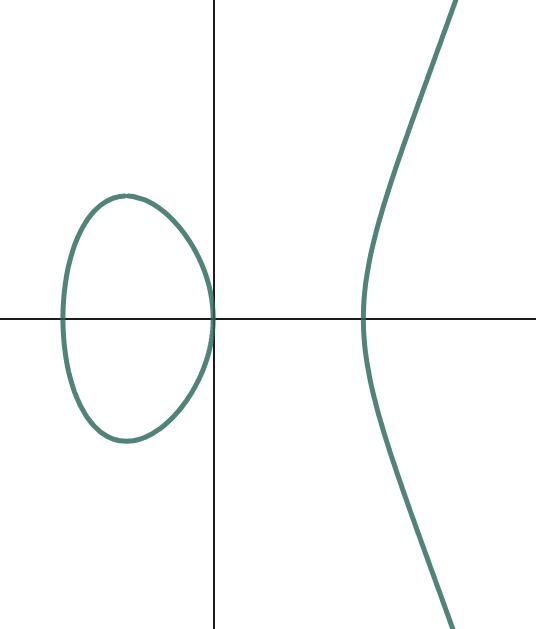
\includegraphics[width=\linewidth]{kap2_bs1.png}
        \caption{Eigene Darstellung mit GeoGebra $y^2=x^3-3x$}
    \end{subfigure}
    \hfill
    \begin{subfigure}{0.45\linewidth}
        \centering
        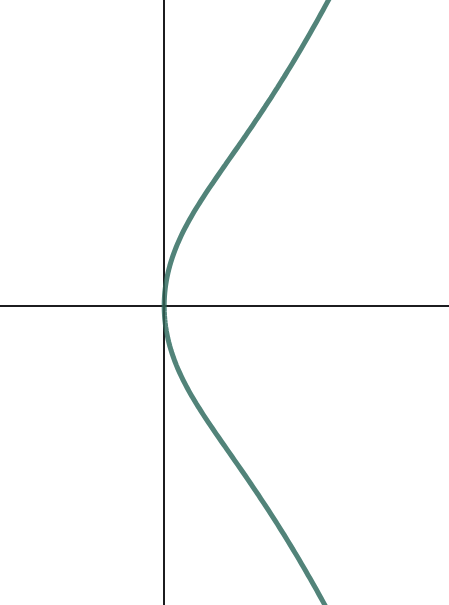
\includegraphics[width=\linewidth]{kap2_bs2.png}
        \caption{Eigene Darstellung mit GeoGebra $y^2=x^3+3x$}
    \end{subfigure}
    \label{fig:vergleich}
    \end{figure}
    Über dem Körper \(\mathbb{R}\) kann die Kurve je nach Anzahl der reellen Nullstellen verschiedene Formen annehmemen. Zum Beispiel hat $y^2 = x^3 - 3x$ drei verschiedene reelle Nullstellen, nämlich $x = 0$ und $x = \pm \sqrt{3}$. Im gegensatz dazu hat die Kurve $y^2 = x^3 + 3x$ lediglich eine reelle Nullstelle bei $x = 0$.\\

    Wie wir in der Darstellung sehen können, ändert sich die Form der Kurve über dem Körper $\mathbb{R}$, wenn wir mehrere reelle Nullstellen haben. Das Polynom \(x^3+Ax+B\) darf daher keine mehrfachen Nullstellen besitzen, dies ist äquivalent dazu, dass die Kurve \emph{nicht singulär} ist.

    \begin{definition}[(Einführung in die algebraische Gemoetrie, S.1+6)]
        Sei $f \in K[x,y]$ und
        \[
        E = V(f) = \{(x,y)\in K^2 \mid f(x,y)=0\}
        \] 
        eine affine ebene Kurve. Ein Punkt \((a,b)\in E\) heißt \textbf{singulär}, wenn,
        \[
        f_x(a,b)=0 \quad \text{und}\quad f_y(a,b)=0.
        \]
         Andernfalls heißt der Punkt \textbf{regulär}.

         Die Kurve \(E\) heißt \textbf{singulär}, wenn sie einen singulären Punkt besitzt.
    \end{definition}
    
    Wir schreiben die Gleichung nun um zu
    \[
    f(x,y)=y^2-x^3-Ax-B
    \]
    dann sind die Ableitung 
    \[
    f_x= -3x^2-A \quad \text{ und } \quad f_y=2y
    \]
    Es muss nun für beide ungleich 0 gelten,
    \[
    f_x= -3x^2-A = 0 \Leftrightarrow 3x^2+A = 0
    \]
    und
    \[
    f_y=2y = 0 \Leftrightarrow y = 0, \quad \text{char }\neq 2
    \]
    daraus folgt ein singulärer Punkt muss die Form $(x,0)$ haben und zusätzlich muss \(x^3+Ax+B = 0\) gelten, sodass der Punkt auf der Kurve liegt. Also x darf nicht eine Nullstelle von \(x^3+Ax+B\) und der Ableitung \(3x^2+A\) sein. Die Diskriminante für ein das kubische Polynom 
    \[
    p(x))x^3+Ax+B
    \]
    ist hierbei
    \[
    \Delta  = -4A^3-27B^2
    \]
   
    \[
        4A^3+27B^2 \neq 0.
    \]
    Für die Nullstellen $r_1, r_2, r_3$ des Polynoms gilt
    \[
    ((r_1 - r_2)(r_1 - r_3)(r_2 - r_3))^2 = -(4A^3 + 27B^2).
    \]
    Insbesondere folgt daraus, dass die Nullstellen genau dann paarweise verschieden sind, wenn die Diskriminante $\Delta = -(4A^3 + 27B^2)$ ungleich Null ist. Im vorliegenden Fall ist $\Delta < 0$, sodass voneinader verschiedene reelle Nullstellen vorliegen.
    
     
    \textbf{Allgemeine Weierstrass Gleichung}
    
    \[y^2+a_1xy+a_3y=x^3+a_2x^2+a_4x+a_6\]


\section{Gruppenstruktur}
Kapitel basier auf \cite{washington08}, S.12ff.
Basiert auch auf (An Introduction to the
Theory of Elliptic Curves, Silverman, S.8-19)
    Wir betrachten nun die Addition von zwei Punkten auf einer Elliptischen Kurve
   
    Wir betrachten dafür zwei Punkte $P=(x_1,y_1)$ und $Q=(x_2,y_2)$ auf einer elliptischen Kurve $E$. Diese ist wie bereits eingeführt gegeben durch die Gleichung \[y^2=x^3+Ax+B.\] Wir wollen nun einen dritten Punkt $P+_EQ=R $ berechnen. Für die graphische Darstellung wurde ein Beispiel über $\mathbb{R}$ verwendet mit der Kurve $y^2=x^3-4x+10$.\\

    Als ersten Schritt zeichnen wir eine Gerade $L$ durch $P$ und $Q$.
    \begin{figure}[htbp]
        \centering
        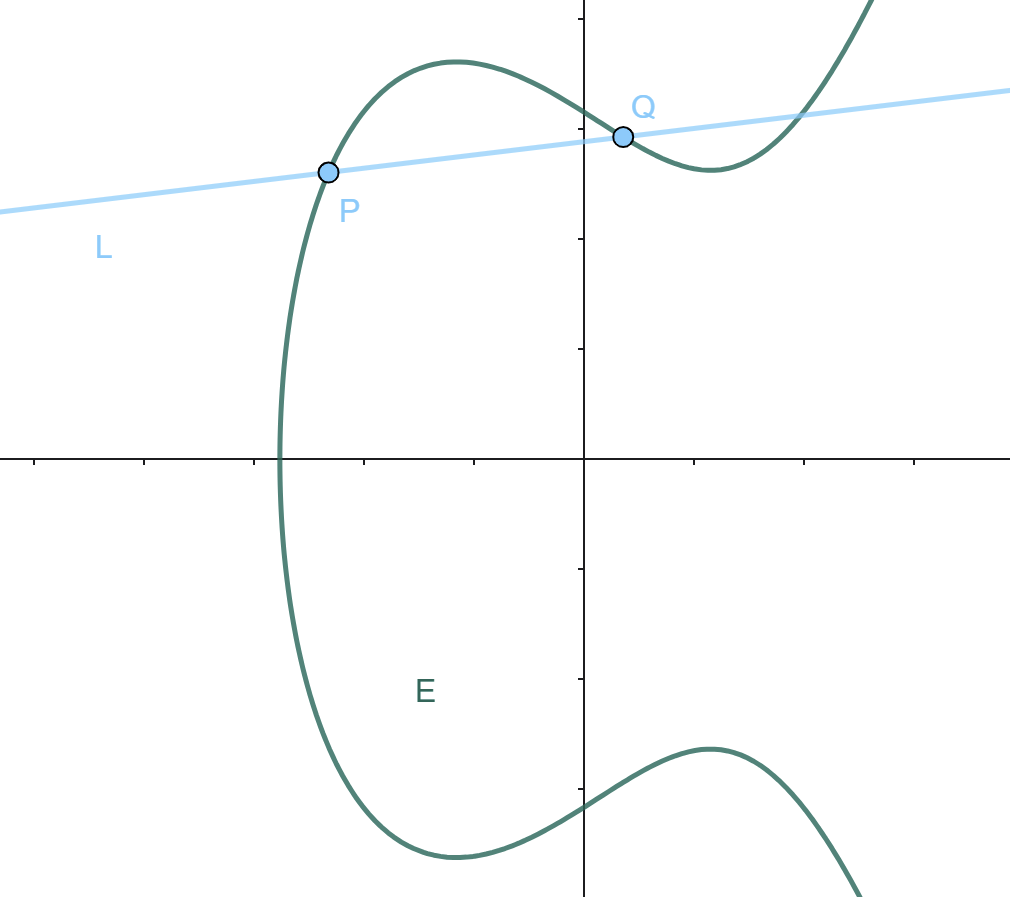
\includegraphics[width=0.5\linewidth]{kap2_2_bsp1.png}
        \caption{Gerade $L$ durch  $P$ und $Q$}
        \label{fig:placeholder}
    \end{figure}

    Als zweiten Schritt nehmen wir den Schnittpunkt $R'$ von der Gerade $L$ und $E$. Anschließend spiegeln wir $R'$ an der x-Achse und erhalten dadurch $R$. Wir definieren $R=P+_E Q$. Hierbei ist wichtig hervorzuheben, dass es sich dabei von der Addition der Koordinaten zweier Punkte unterscheidet.

    \begin{figure}[htbp]
        \centering
        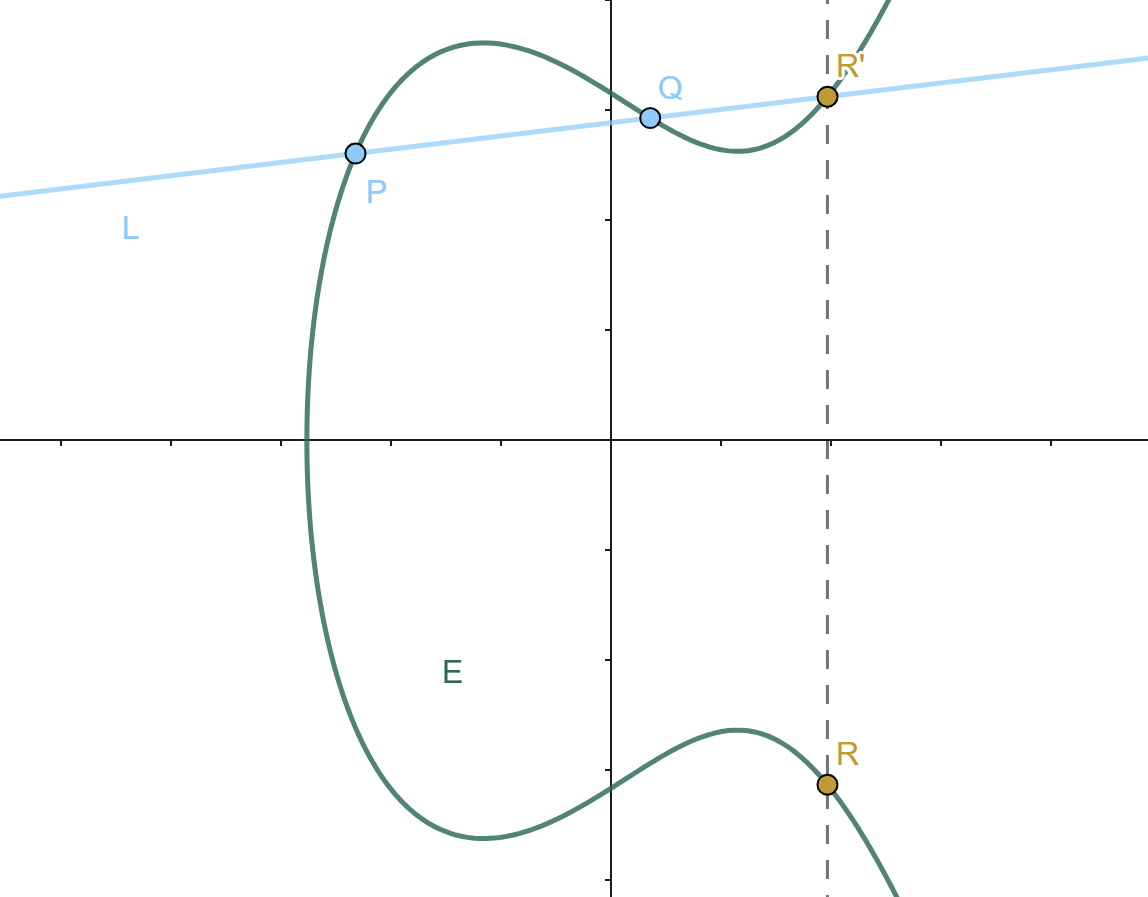
\includegraphics[width=0.5\linewidth]{kap2_2_bsp2.png}
        \caption{Schnittpunkt $R'$ von Gerade $L$ und Kurve $E$ und die Spiegelung $R$}
        \label{fig:placeholder}
    \end{figure}

    Nun betrachten müssen wir noch den Fall betrachten, wenn wir einen Punkt $P$ auf sich selbst addieren wollen auf der Kurve $E$. Da es keinen zweiten Punkt, sodass durch beide Punkte eine Gerade gezogen werden kann, nehmen wir an der zweite Punkt $Q$ nähert sich P an, sodass die Gerade $L$ zu einer Tangente von $E$ bei $P$ wird.
    \begin{figure}[htbp]
        \centering
        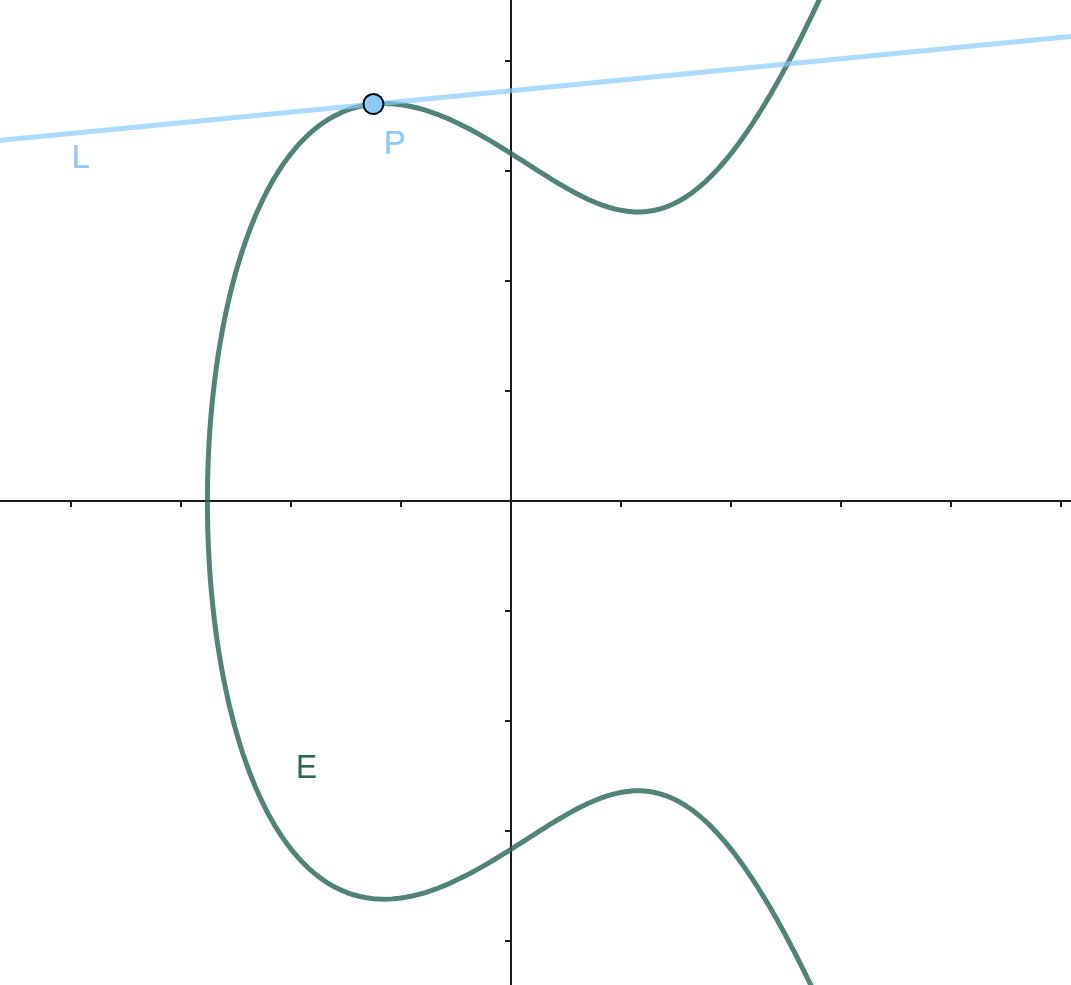
\includegraphics[width=0.5\linewidth]{kap2_2_bsp3.png}
        \caption{Tangente am Punkt $P$}
        \label{fig:placeholder}
    \end{figure}
    
    Anschließend nehmen wir wieder den Schnittpunkt $R'$ von der Kurve $E$ und der Tangente $L$ und spiegeln diesen an der x-Achse. Dadurch erhalten wir wieder den Punkt $P+_EP=R$, denn wir aber nun als $2P$ bezeichnen.

    \begin{figure}[htbp]
        \centering
        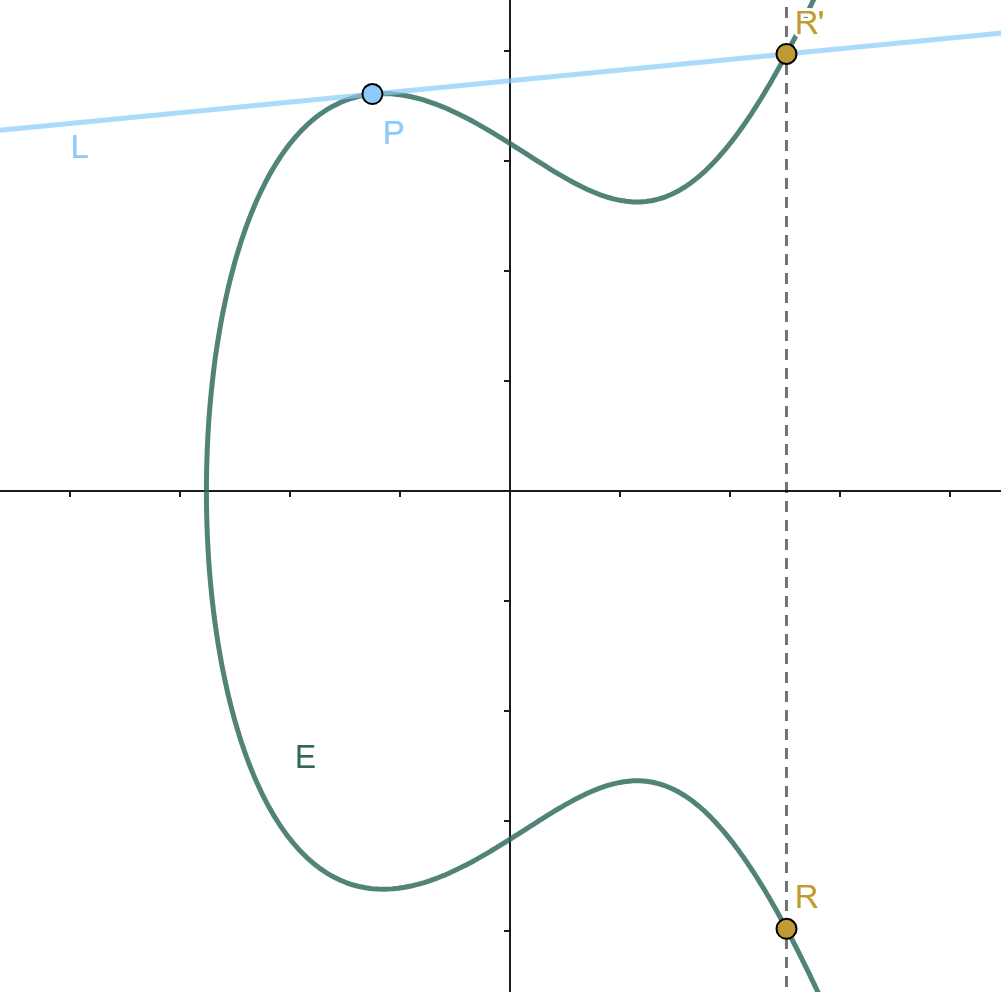
\includegraphics[width=0.6\linewidth]{kap2_2_bsp4.png}
        \caption{piegelung von $R'$, wodurch $R=2P$ entsteht}
        \label{fig:placeholder}
    \end{figure}
    
    Als letzten Fall schauen wir uns noch an, wenn die Gerade $L$ keinen Schnittpunkt mit $E$ hat. Hierfür betrachten wir wieder den Punkt $P$ und seinen an der x-Achse gespiegelten Punkt $P'=-P$.
    \begin{figure}[htbp]
        \centering
        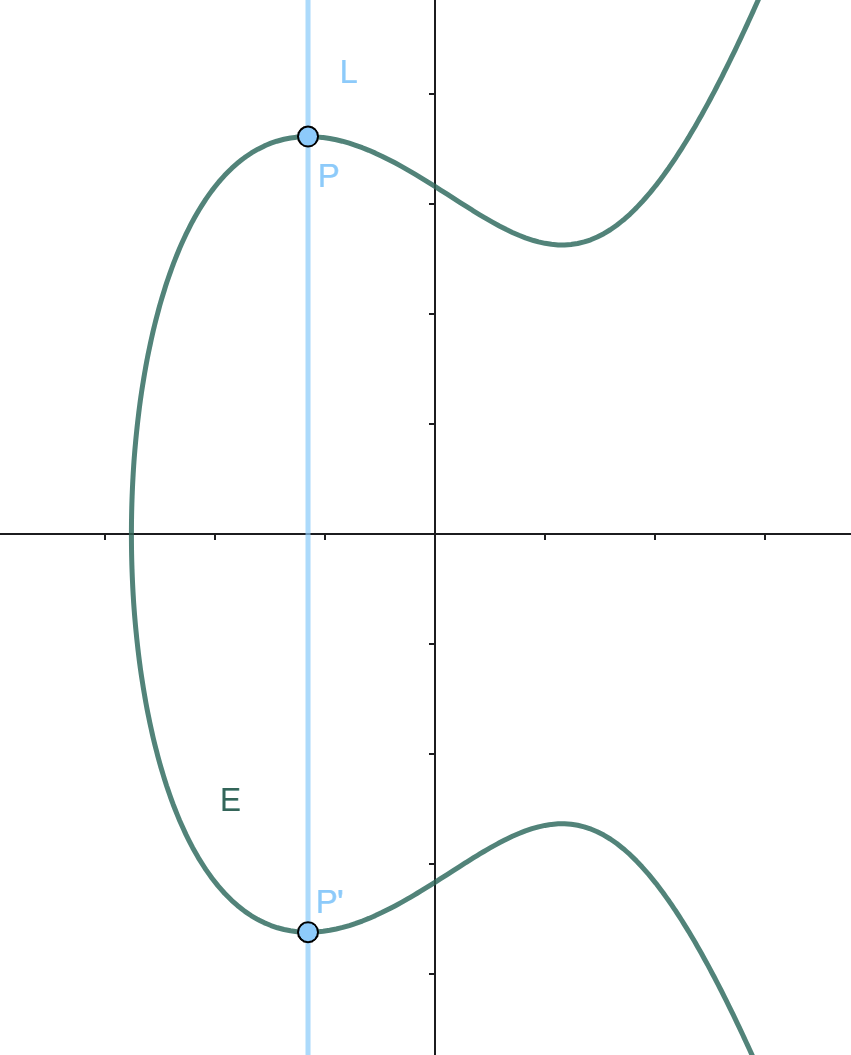
\includegraphics[width=0.5\linewidth]{kap2_2_bsp5.png}
        \caption{Schnittpunk von L im Punkt $\infty$}
        \label{fig:placeholder}
    \end{figure}
    Dafür brauchen wir einen dritten Punkte um $P+_E(-P)$ definieren zu kennen wir kreieren dafür einen Punkt $\infty$. Dieser Punkt ist dabei auf jeder vertikalen Gerade.\\

    \textbf{Herleitung der Additionsformeln
    \cite{washington08}(, S. 14 und Kaplan S.179ff.):}\\
    (Bei diesem Absatz habe ich mich orientiert an 
Kryptographie, Buell, S.99)
       
     Seien nun $P=(x_1,y_1)$ und $Q=(x_2,y_2)$ Punkte auf $E$ mit $P,Q\neq \infty$.
    Zuerst betrachten wir den Fall $P\neq Q$ und \(x_1\neq x_2\). Dann hat die Gerade \(L\) durch durch \(P\) und \(Q\) die Form
    \[
    y=m(x-x_1)+y_1
    \qquad \text{mit} \qquad
    m=\frac{y_2-y_1}{x_2-x_1}.
    \]
    Zur Bestimmung des dritten Schnittpunkts setzen wir die Geradengleichung in die Kurvengleichung
    \[
    E: y^2=x^3+Ax+B
    \]
    ein. Es gilt also
    \[
    \bigl(m(x-x_1)+y_1\bigr)^2=x^3+Ax+B.
    \]
    Nach Ausmultiplizieren und Umstellen erhält man
    \[
    0=x^3-m^2x^2+\bigl(2m^2x_1-2my_1+A\bigr)x
    +\bigl(B-m^2x_1^2+2mx_1y_1-y_1^2\bigr).
    \]
    
   Die Nullstellen des kubischen Polynoms sind die \(x\)-Koordinaten der drei Schnittpunkte von \(L\) mit \(E\), also \(x_1\), \(x_2\) und \(x_3'\). Daher gilt
    \[
    0=(x-x_1)(x-x_2)(x-x_3')
    =x^3-(x_1+x_2+x_3')x^2+(x_1x_2+x_1x_3+x_2x_3)x-x_1x_2x_3
    \]
    Mit Kooeffizientenvergleich erhält man
    \[
    x_1+x_2+x_3' = m^2 \Leftrightarrow  x_3' = m^2-x_1-x_2
    \]
    Da \(R'=(x_3',y_3')\) auf der Geraden \(L\) liegt, gilt
    \[
    y_3'=m(x_3'-x_1)+y_1.
    \]
    Die Summe \(P+Q\) ist die Spiegelung von \(R'\) an der \(x\)-Achse. Somit ist
    \[
    P+Q=(x_3,y_3)
    \]
    mit
    \[
    x_3=x_3'=m^2-x_1-x_2,
    \qquad
    y_3=-y_3'=m(x_1-x_3)-y_1.
    \]    
    
    \textbf{voll restliche Herleitung Einfügen, Rosen S.12-14}
    
    Dann definieren wir $P+Q=R=(x_3,y_3)$ wie folgt:
    \begin{enumerate}
        \item Wenn $x_1\neq x_2$, dann
        \[x_3=m^2-x_1-x_2, \quad y_3=m(x_1-x_3)-y_1 \quad \text{ mit  } m=\frac{y_2-y_1}{x_2-x_1}.\]
        \item Wenn $x_1=x_2$, aber $y_1\neq y_2$, dann ist 
        \[P+Q=\infty.\]
        \item Wenn $P=Q$ und $y_1\neq 0$, dann
        \[x_3=m^2-2x_1, \quad y_3=m(x_1-x_3)-y_1, \quad \text{ mit } m=\frac{3x_1^2+A}{2y_1}.\]
        \item Wenn $P=Q$ und $y_1=0$ dann, 
        \[P+Q=\infty.\]
    \end{enumerate}

    Zusätzlich definieren wir 
    \[P+\infty=P\]
    für alle Punkte $P$ auf $E$.Damit ist $E(L)$ geschlossen unter Addition von Punkte auf der Kurve. 

    \begin{theorem}
        Die Addition auf einer Elliptische Kurve $E$ erfüllt folgende Eigenschaften.
        \begin{enumerate}
            \item [Existenz der Identität:] \(P+\infty=\infty+P=P\) für alle \(P\in E\)
            \item [Kommutativität:] \(P+Q=Q+P\) für alle \(P,Q\in E\)
            \item [Existenz des Inversen:] Sei $P\in E$ gegeben, dann exestiert ein $-P\in E$ mit \(P+(-P)= \infty\), für alle $P\in E$.
            \item [Assoziativität:] \((P+Q)+R=P+(Q+R)\) für alle \(P,Q,R\in E\)
        \end{enumerate}
    \end{theorem}
    Damit formen alle Punkte auf $E$ eine additive abelsche Gruppe mit $\infty$ als neutrales Element.

\begin{proof}
    Die Existenz der Identität ist durch die Definition der Elliptische Kurve gegeben. Die Kommutativität kann einfach nachgerechnet werden indem die oben definieren Regeln für die Addition zweier Punkte anwenden.
    Für  das Inverse müssen wir von einem Punkt $P$ sein Reflektion an der x-Achse $P'$ nehmen. Dann erhalten wir $P+P'=\infty.$
    Der Beweis der Assoziativität ist recht langwierig und daher wird auf eine externe Quellen hierfür verwiesen \textbf{Quelle für Assoziativität einfügen, Potenziell (\cite{washington08},S.20ff. Proof of Associativity}
\end{proof}


\textbf{Beispiel 1:}
    Wir betrachten dafür eine Elliptische Kurve $E$ mit 
    \[y^2=x^3-4x+4,\]
    auf dieser Kurve liegen zum Beispiel die Punkte $P=(0,2)$ und $Q=(2,2)$. Nun berechnen wir auf den vorherigen Regeln, da $x_1\neq x_2$ folgt,
    \[
        m = \frac{2-2}{2-0}=0
    \]
    \[
        x_3 = (0)^2-0-2=-2, \quad  y_3 = 0\cdot(0-(-2))-2 =-2
    \]
    also
    \[
    P+_EQ=(0,0)+_E(0,2)= (-2,-2)
    \]
    Analog können wir beliebige Punkte auf der Kurve addieren.
    \[(0,2)+_E(-2,-2)=(6,14)\]

    
    \textbf{Beispiel 2:}
    Nun können wir auch Punkte berechnen, wenn wir diese geometrisch nicht sinnvoll darstellen können. Die Kurve \(y^2=x^3-4x+4\pmod 7\) also über dem endlichen Körper $\mathbb{F}_7$. (Als Errinnerung die Kurve muss über dem Körper Singulär sein\(4A^3+27B^2=4\cdot(-4)^3+27\cdot4^2=176\equiv1\pmod 7\neq0\)

    Wir wählen nun die Punkte $P=(0,2)$ und \(Q=(5,5)\)
    auf $E(\mathbb{F})_7$.
    Es gilt nun 
    \[
    m=\frac{5-2}{5-0}=\frac{3}{5} = 3\cdot 5^{-1}\equiv 3\cdot 3 \pmod 7= 9 = 2 \pmod 7
    \]
    und damit
    \[
    x_3=2^2-0-5=-1\equiv 6 \pmod 7, \quad y_3=2(0-6)-2=-14 \equiv 0\pmod 7
    \]
    also
    \[P+_EQ=(6,0).\]

    
    \textbf{Skalar mal Punkt}(The aglebra of Elliptic Curves, S.30f.)
    Um später Diffie-Hellman über der endlcihen Gruppe $E(\mathbb{F}_p)$ anwenden zu können(wird im Kryptographie Kapitel genauer erklärt), muss man auch für größere $p$ berechnen können, also
    \[mP=P+P+\dots+P\in E(\mathbb{F}_p)\] für sehr große Werte von m.
    Lass \(m\in\mathbb{N}_{>0}\).

    Wir schreiben zuerst 
    \[m=m_0+m_1\cdot2+m_2\cdot 2^2+\dots+m_r\cdot 2^r, \quad m_0,\dots,m_r\in\{0,1\}\]
    also zerlegen m in seinen einzelnen Zweierpotenzen. Dann kann $mP$ berechnet werden als
    \[mP=m_0P+m_1\cdot 2P+m_2\cdot2^2P+\dots +m_r\cdot 2^rP,\]
    wobei \(2^kP=2\cdot 2\cdots 2P\) benötigt nur k Doppelungen und damit können wir $mP$ in $O(\text{log } m)$ berechnen. Die Binärdarstellung von $m$ hat 
    \[
    r+1 = \lfloor\log_2m \rfloor+1
    \].
    Im Schnitt braucht man also $\log_2(m)$ Verdoppelungen und \(\frac{1}{2}\log_2(m)\) Additionen um $mP$ zu berechnen.

    Man kann die benötigte Zeit nochmal reduzieren, indem man die Non-Adjacent Form verwendet. Die Addition und Subtraktion eines Punktes kosten genau gleich viel Zeit, also schreiben wir
    \[
    m=m_0+m_1\cdot 2+m_2\cdot 2^2+\cdots+m_r\cdot 2^r, \quad m_0,\dots,m_r\in\{-1,0,1\}.
    \]
    Hierfür können wir im Schnitt  $\frac{2}{3}$ der $m_i=0$ für die Zerlegung nutzen, dass reduziert die Anzahl der durchschnittlichen Additionen auf \(frac{1}{3}\log_2(m)
    \).
    Aufgrund dieses Vorgehens ist die Berechnung von $m$ aus $P$ und $mP$ sehr schwierig. Das sogennante \textbf{diskrete Logarithmus Problem} für Elliptische Kurven ist später essenziell für das kryptographische Verfahren, das auf diesen aufbaut.
   

\section{Projektiver Raum und der Punkt bei Unendlich} (vgl. \cite{washington08}, S. 18ff.)
(vgl. \cite{clader25}, S.245f.)
    
    Die Gruppenstruktur elliptischer Kurven wurde zuvor über die geometrische
    Punktaddition beschrieben. Dabei spielt der Punkt im Unendlichen eine besondere
    Rolle, da er als neutrales Element der Gruppe dient. Um diesen Punkt geometrisch
    präzise zu beschreiben, gehen wir nun von der affinen Ebene zur projektiven Ebene über. 

    \begin{definition}[Projektive Ebene]
    Sei \(K\) ein Körper. Die projektive Ebene über \(K\) ist definiert als der Quotient
    \[
    \mathbb P^2_K
    =
    \left(K^3\setminus0\right)/\sim,
    \]
    wobei zwei Tripel \((x,y,z),(x',y',z')\in K^3\setminus\{(0,0,0)\}\) genau dann in einer Relation  stehen \(
    (x,y,z)\sim (x',y',z)\), wenn ein \(\lambda\in K^\times:
    (x,y,z)=\lambda(x',y',z')\) exestiert.
    Die Äquivalenzklasse von \((x,y,z)\) wird mit
    \((x:y:z)\) bezeichnet und heißt Punkt der projektiven Ebene.
    \end{definition}
    Die Koordinaten \((x:y:z)\) werden homogene Koordinaten genannt. Dabei bezeichnet \((x:y:z)\) nicht einen einzelnen Punkte, sondern die Äquivalenzklasse aller von Null verschiedenen skalaren Vielfachen von \((x,y,z)\). Für jedes \(\lambda\in K^\times\) gilt also
    \[
    (x:y:z)=(\lambda x:\lambda y:\lambda z).
    \]
     Die Menge 
    \[
    g_\infty=\{(x:y:z)\in \mathbb P^2_K\mid z=0\}.
    \]
    heißt die unendlich ferne Gerade der projektiven Ebene (vgl. \cite{forster15}, S.200ff.).
    Ist $z \neq 0$, so kann z auf 1 normiert werden, denn es gilt \((x:y:z)=(x/z:y/z:1)\). Nun kann man eine Abbildung definieren
    \[
    K^2\longrightarrow\mathbb{P}^2_K, \quad
    (x,y)\mapsto (x:y:1).
    \]
    Diese Punkte entsprechen genau den affinen Punkten \((x,y)\in K^2\) die bijektiv auf \(\mathbb{P}^2_K\setminus g_\infty\) abgebildet werden.


    \begin{lemma}
        Die Punkte auf der Geraden im Unendlichen \(L_\infty\) entsprechen den RIchtungen affiner Geraden. Insbesondere schneiden sich parallel affine Geraden in der projektiven Ebene in demselben Punkt auf \(L_\infty\).
    \end{lemma}
    Ich weiß nicht ganz wie ich das definieren soll.

    Soll ich auch definieren, dass es sich um eine Äquivalenzklasse handelt?
\section{Beweis der Assoziativitität}
    Beweis nach vgl. \cite{zwegers24}, S. 477ff.
    Es gibt hierbei gibt es 3 Sonderfälle, erstens die Punkte könnten in unendlich liegen, dafür brauchen wir die projektiven Koordinaten. Zweitens die Gerade könnte eine Tangente bei E sein, was bedeutet, dass zwei Punkte gleich sind. Drittens zwei Geraden könnten gleich sein.
    Wir möchten nun die Assoziativität zeigen. Sei \(E=y^2=x^3+Ax+B\) eine elliptische Kurven über einem Körper \(K\) mit \(\text{char(K)}\neq 2,3\) und \(4A^3+27B^2 \neq 0\).
    Weiter seien nun die Punkte\[
    P_1=(x_1,y_1),\quad P_2=(x_2,y_2),\quad P_3=(x_3,y_3)
    \]
    Punkte aus \(E\setminus\{O\}\). Ziel ist es zu zeigen, dass
    \[
    (P_1+P_2)+P_3=P_1+(P_2+P_3)
    \]
    gilt.

   Für zwei Punkte \(P_i=(x_i,y_i)\) und \(P_j=(x_j,y_j)\) mit
    \(P_j\neq -P_i\) setzen wir
    \[
    \alpha(P_i,P_j):=
    \begin{cases}
    \dfrac{y_j-y_i}{x_j-x_i}, & \text{falls } x_i\neq x_j,\\[1.2ex]
    \dfrac{3x_i^2+A}{2y_i}, & \text{falls } P_i=P_j \text{ und } y_i\neq 0.
    \end{cases}
    \]
    Wir suchen nun eine Parabel durch \(P_1,P_2,P_3\). Wir finden dafür einen neuen Punkt \(P_4=(P_1+P_2)+P_3\), definiert mit
    \[
    x_4=-x_1+x_2-x_3+\frac{1}{c_2^2}-2\frac{c_1}{c_2}, \quad y_4 = -y_2-(x_4-x_2)(c_1+x_4c_2)
    \]
    wobei 
    \[
    c_1 := \frac{x_1\alpha(P_2,P_3)-x_3\alpha(P_1P_2)}{x_1-x_3}, \quad c_2:=\frac{\alpha(P_1,P_2)-\alpha(P_2,P_3)}{x_1-x_3}.
    \]

   
    

\section{Elliptische Kurven in Charakteristik 2} (nach Rosen, S. 47ff.) \textbf{Muss man hier auch characteristik 3 ergänzen?}

    Computer arbeiten tendenziell besser über Körpern der Charakteristik 2 im Vergleich zu Körpern mit großen prim Charakteristiken.Daher werden häufig Elliptische Kurven über einem Feld $\mathbb{F}_q$ mit $q=2^k$ Elementen verwendet.
    (vgl. \cite{silverman06}, S.47)

    Aus dieser Notwendigkeit betrachten wir nun genauer Elliptische Kurven in Charakteristik 2, da hier einige unserer vorher definierten Formeln nicht funktionieren.\\
    \begin{satz}
         In Charakteristik \(2\) ist die kurze Weierstrass Gleichung \(y^2=x^3+Ax+B\) stets singulär. Daher verwendet man in Charakteristik 2 die allgemeine Weierstraß-Gleichung
    \end{satz}

    \[
    y^2+a_1xy+a_3y=x^3+a_2x^2+a_4x+a_6.
    \]
    \begin{proof}    
        Betrachte 
        \[
        f(x,y) = y^2-x^3-Ax-B.
        \]
        Ein Punkt auf der Kurve ist genau dann singulär, wenn beide partiellen Ableitungen verschwinden. Es gilt
        \[
        f_y=2y\equiv0,
        \] da der Körper Charakteristik 2 hat. Außerdem ist 
        \[
        f_x=-3x^2-A
        \]
        Sei nun $x_0$ eine Nullstelle von $f_x$. Wir wählen ein \(y_0\) mit
        \[
        y_0^2=x_0^3+Ax_0+B
        \]
        Dann liegt $(x_0,y_0)$ auf der Kurve und es ist
        \[
        f_x(x_0,y_0)=f_y(x_0,y_0) = 0
        \]
        Damit folgt die Kurve ist singulär.
    \end{proof}
    
    Nun wollen auch für Charakterstik 2 die Gruppengesetze aufstellen.
    Hierfür beginnen wir mit der allgmeinen Weierstraß-Gleichung für eine elliptische Kurv $E$
    \[
    y^2+a_1xy+a_3y=x^3+a_2x^2+a_4x+a_6.
    \]
    Man schreibt diese in die Form
    \[
    f(x,y)=y^2+a_1xy+a_3y-x^3-a_2x^2-a_4x-a_6.
    \]
    Dann sind die partiellen Ableitungen gegeben durch
    \[
    f_x=a_1y-3x^2-2a_2x-a_4,\qquad f_y=2y+a_1x+a_3.
    \]
    In Charakteristik \(2\) vereinfacht sich dies zu
    \[
    f_x=a_1y+x^2+a_4,\qquad f_y=a_1x+a_3.
    \]
    Ein Punkt \((x,y)\) ist wie bereits früher eingeführt, genau dann singulär, wenn
    \[
    f(x,y)=0,\qquad f_x(x,y)=0,\qquad f_y(x,y)=0.
    \]
    Fall 1: $a_1\neq 0$
    Man kann aus \(a_1x+a_3=0\) folgern
    \[
    x=\frac{a_3}{a_1}.
    \]
    Eingesetzt in \(a_1y+x^2+a_4=0\) liefert es,
    \[
    a_1y+\left(\frac{a_3}{a_1}\right)^2+a_4=0
    \]
    \[
    y= \frac{a_3^2}{a_1^3}+ \frac{a_4}{a_1}.
    \]
    wenn der Punkt zusätzlich \(f(x,y)=0\) erfüllt handelt es sich um einen singulären Punkt.
  
    Fall 2: $a_1=0$
    Es gilt nun,
    \[
    f_x=x^2+a_4,\qquad f_y=a_3.
    \]
    also muss \(a_3= 0\) und $f(x,y)=0$ gelten, sodass $(x,y)$ ein singulärer Punkt ist.\\

    Nun können wir die Addition von Punkten definieren. Es gilt wieder für alle Punkte $P\in E$
    \[
    P+\infty=P.
    \]
    \textbf{washington S.48-49 hier weiter machen}


\chapter{Elliptische Kurven über endlichen Körpern}
Für die algebraischen Grundlagen wird \cite{karpf24}, S.317-318 verwendet.
\section{Motivation}
Nicht jede Art von elliptischer Kurve macht Sinn im Bereich der Kryptography. Zum Beispiel würden Kurven über reellen Zahlen Gleitpunkt Arithmetik benötigen, welche Probleme wie Ungenauigkeit oder verringerte Rechenleistung mit sich bringen würden. Daher werden elliptische Kurven über endlichen Körpern definiert.
Hierbei wird wie bereits eingeführt die kurze Weierstraß-Gleichung verwendet(vgl. \cite{omondi20}, S.230). Man benötigt für Kapitel 5 sichere Kurven, daher muss man gewisse Dinge über die Ordnung und Eigenschaften erfahren.

\section{Endliche Körper}
\begin{definition}
    Ein endlicher Körper ist ein Körper mit endlich vielen Elementen. Für jede Primzahlpotenz \(q=p^n\) existiert bis auf Isomorphie genau ein endlicher Körper mit \(q\) Elementen. Dieser wird dann mit \(\mathbb F_q\) oder \(GF(q)\)(Galois Field) bezeichnet.
\end{definition}
In kryptographischen Anwendungen treten insbesondere die Körper \(\mathbb F_p\) und \(\mathbb F_{2^m}\) auf. Der kleinste Durchscnitt $P$ aller Teilkörper von $K$ wird der \textbf{Primkörper} genannt
\[
    P=\cap \{U|U \text{ist ein Teilkörper von }K\}.
\]
\begin{satz}

    \label{hilfs:primkörper}
    Seien $K$ ein Körper und $K_0$ der Primkörper von $K$.
    \begin{enumerate}
        \item Ist char($K)=0$, so ist $K_0$ zu $\mathbb{Q}$ isomorph.
        \item Ist char($K)=p\neq 0$, so ist $K_0$ zu $\mathbb{Z}/p\cdot \mathbb{Z}$ isomorph.
    \end{enumerate}
\end{satz}
Mit Worten heißt dies: Hat $K$ die Charakteristik 0, so ist der Primkörper von $K$ zu $\mathbb{Q}$ isomorph. Ist die Charakteristik $p \neq 0$, so ist er zu $\mathbb{Z}/p$ isomorph.
\begin{proof}
    \begin{enumerate}
        \item Sei \(\Phi:\mathbb{N}\leftarrow K_0\) eine Abbildung für alle $n\in\mathbb{N}$. Sei
              \[
                  n^\Phi = (1_k+\cdots+1_k). \quad \text{n-mal}.
              \]
              Sind $n,m\in\mathbb{N}$ und $n\leq m$ mit der Eigenschaft $n^\psi=m^\psi$, so folgt
              \[
                  0_K=n^\psi-m^\psi=(1_K+\cdots+1_K). \quad \text{(n-m)-mal}.
              \]
              Da char($K)=0$. ist ist, dann $n=m$. Also ist $\psi$ eine injektive Abbildung. Somit besitzt jede $K_0$ eine Teilmenge, die sich bezüglich der Addition wie $\mathbb{N}$ verhält. Da $K_0$ ein Körper ist, gibt es also in $K_0$ einen zu $\mathbb{Z}$ isomorphen Teilring und dann auch einen zu $\mathbb{Q}$ isomorphen Teilkörper. Da $\mathbb{Q}$ keine echten Teilkörper hat, ist $K_0$ selbst isomorph zu $\mathbb{Q}$.
        \item Seien nun $p$ eine Primzahl und char($K)= p$. Sei weiter
              \[
                  L = {0_K,1_K,\dots,1_k+\cdots+1_K}\quad \text{(p-1)-mal}
              \]
              Da char($K)=p$ ist, sind die Elemente in $L$ paarweise verschieden und daher ist $|L|=p$, außerdem ist $L$ unter Addition abgeschlossen.

    \end{enumerate}
\end{proof}
\cite{stroth24}, S.66--67
\begin{satz}
    Sei $K$ ein endlicher Körper. Dann gibt es eine Primzahl $p$ und ein $n\in \mathbb{N}$, sodass \(|K|=p^n\) ist.
\end{satz}

\begin{proof}
    Da \(K\) endlich ist, müssen in der Folge
    \[
        0,\ 1_K,\ 1_K+1_K,\ 1_K+1_K+1_K,\ \dots
    \]
    zwei Elemente übereinstimmen. Daher gibt es eine kleinste positive
    natürliche Zahl \(p\) mit
    \[
        p\cdot 1_K=0.
    \]
    Diese Zahl ist die Charakteristik von \(K\).

    Die Zahl \(p\) ist eine Primzahl. Wäre nämlich \(p=rs\) mit
    \(1<r,s<p\), so wäre
    \[
        (r\cdot 1_K)(s\cdot 1_K)=p\cdot 1_K=0.
    \]
    Da ein Körper keine Nullteiler besitzt, müsste
    \(r\cdot 1_K=0\) oder \(s\cdot 1_K=0\) gelten. Dies widerspricht
    der Minimalität von \(p\).

    Der von \(1_K\) erzeugte Primkörper besitzt somit \(p\) Elemente
    und ist isomorph zu \(\mathbb{F}_p\). Folglich ist \(K\) ein
    Vektorraum über \(\mathbb{F}_p\). Da \(K\) endlich ist, besitzt
    dieser Vektorraum eine endliche Dimension \(n\).

    Bezüglich einer Basis besitzt jedes Element von \(K\) eine
    eindeutige Darstellung
    \[
        a_1v_1+\dots+a_nv_n
        \qquad\text{mit }a_i\in\mathbb{F}_p.
    \]
    Für jeden der \(n\) Koeffizienten gibt es \(p\) Möglichkeiten.
    Daher gilt
    \[
        |K|=p^n.
    \]
\end{proof}

\cite{stroth24},S.163

\(|K|=p^n\), wenn $n$ der Grad von $K$ über dem nach Lemma 21.1 (b) zu $\mathbb{Z}/p$ isomorphen Primkörper.

\begin{lemma}
    Für einen endlichen Körper K der Charakteristik p gilt und $q=p^n$
    \[
        a^q=a
    \] für jedes $a\in K$.
\end{lemma}

\begin{proof}
    Für \(a=0\) ist die Aussage unmittelbar erfüllt, da $0^{p^n}=0$. Sei daher \(a\in K^\times =K\setminus\{0\}\).
    Wegen $|K^\times|=p^{n-1}$ gilt nach dem kleinen Satz von Fermat vgl. \cite{karpf24} S.46 gilt  in einer endlichen Gruppe $G$, \(a^{|G|} = e\) für alle \(a\in G\). Dann \(a^{p^n-1}=1\) für jedes $a\in K^\times$. Daraus folgt dann $a^{p^n}=a$ für alle $a\in K $.
\end{proof}

(vgl. \cite{karpf24}, S.391--392)
Diese Aussage kann nun auch noch in beide Richtungen formuliert werden, da wir sie später bei einem Beweis benötigen.
\begin{lemma}
    Für \(a\in \overline{\mathbb{F}}_q\) gilt
    \[
        a^q=a\Leftrightarrow a\in\mathbb{F}_q
    \]
\end{lemma}
\begin{proof}
    Nach dem vorherigen Lemma gilt für jedes
    \(a\in\mathbb F_q\), dass \(a^q=a\), also
    \(a^q-a=0\). Somit sind die \(q\) Elemente von
    \(\mathbb F_q\) verschiedene Nullstellen des
    Polynoms \(f(X)=X^q-X\).

    Da \(f\) den Grad \(q\) besitzt, hat es auch über
    dem algebraischen Abschluss \(\overline{\mathbb F}_q\)
    höchstens \(q\) verschiedene Nullstellen. Seine
    Nullstellen sind daher genau die Elemente von
    \(\mathbb F_q\). Folglich gilt für jedes
    \(a\in\overline{\mathbb F}_q\):
    \[
        a^q=a \quad\Longleftrightarrow\quad a\in\mathbb F_q.
    \]
\end{proof}


\begin{definition}[Elliptische Kurve über \(\mathbb F_p\)]
    Sei \(p>3\) eine Primzahl. Eine elliptische Kurve über \(\mathbb F_p\) ist die Menge von allen Punkten $(x,y)\in \mathbb{F}_p$ mit
    \[
        \mathbb F_p = y^2 \equiv x^3+ax+b \pmod p
    \]
    und einem Punkt im Unendlichen.
    \[
        4a^3+27b^2 \not\equiv 0 \pmod p
    \] gilt. Die Bedingung stellt wie im allgemeinen Fall sicher, dass die Kurve nichtsingulär ist. Die Einschränkung $p>3$ erlaubt die Verwendung der kurzen Weierstraß-Gleichung. Für Körper der Charakteristik \(2\) und \(3\) haben wir bereits in Kapitel 3 gesehen, dass die allgemeine Weierstraß-Gleichung verwendet werrden muss.
\end{definition}
(\cite{guneysu24},S.279f.)
\begin{theorem}
    Sei $\mathbb{F}_q$ ein endlicher Körper, dann ist die Gruppe der Punkte $E(\mathbb{F}_q)$ immer eine zyklische Gruppe oder das Produkt von zwei zyklischen Gruppen.
\end{theorem}

\cite{silverman06}, S.29

\begin{proof}

\end{proof}

\section{Die Punktmenge $E(\mathbb{F}_q)$}

\subsection{Explizite Punktbestimmung}
\cite{washington08},S.95, hier noch eigene Beispiele erstellen
\begin{enumerate}
    \item Sei E die Kurve $y^2=x^3+x+1$ über $\mathbb{F}_5$. Um nun die Punkte von E zu erhalten, berchnen wir zuerst $x^3+x+1\mod 5$ und anschließend die quadratwurzel von diesem Polynom über $F_5$.
          \begin{center}
              \begin{tabular}{c|c|c|c}
                  x & $x^3+x+1$ & y       & Points       \\
                  \hline
                  0 & 1         & $\pm$ 1 & (0,1), (0,4) \\
                  1 & 3         & -       & -            \\
                  2 & 1         & $\pm$ 1 & (2,1),(2,4)  \\
                  3 & 1         & $\pm 1$ &              \\
                  4 & 4         & $\pm 2$ & (4,2),(4,3)
              \end{tabular}
          \end{center}
          Beachte: $-1\equiv 4 \mod 5$ und $ -2\equiv 3 \mod 5$\\
          Für $y^2=3$ gibt es keine Wurzel in $F_5$\\

          Also ist nun die Ordnung:
          \[
              \mid E(\mathbb{F}_5)\mid = \# \{(x,y)\in \mathbb{F}_5 \mid y^2=x^3+x+1\}+1 = 9
          \]
          Wir berechnen nun einen Punkt  $(3,1)+(2,4)$ auf $E$:
          \[
              \frac{4-1}{2-3}=\frac{3}{-1}=\frac{3}{4}=3\cdot4^{-1} =3\cdot 4=12  \equiv 2 \mod 5
          \]
          Es ist also $y=2(x-3)+1\equiv 2x$. Wenn wir dass nun in die Gleichung für die Kurve einsetzen erhalten wir
          \[(2x)^2=x^3+x+1\Leftrightarrow 0 = x^3-4x^2+x+1\]. Wir kennen schon zwei Schnittpunkte der Kurve $x=3$ und $x=2$, da $(3,1)$ und $(2,4)$ auf der Gerade und Kurve liegen. Da das Polynom kubisch ist, muss die Summe der drei Nullstellen 4 sein. Damit gilt,
          \[
              3+2+r \equiv 4 \mod 5 \Leftrightarrow r\equiv 4 \mod 5
          \]
          Also ist die dritte Koordinate $x=4$, nun erhalten wir $y=2x\equiv 3$, gespiegelt über die x-Achse erhält man die Summe
          \[(3,1)+(2,4)=(4,2)\]

\end{enumerate}




\begin{theorem}
    Sei $E$ eine elliptische Kurve über einem endlichen Körper $\mathbb{F}_q$. Dann gilt,
    \[
        E(\mathbb{F}_q) \simeq \mathbb{Z}_n \text {  oder  } \mathbb{Z}_{n_1} \oplus \mathbb{Z}_{n_2}
    \]
    für ein $n \geq 1$ und für beliebige $n_1,n_2\geq1$ mit $n_1\mid n_2$.
\end{theorem}
\begin{proof}
    Aus der Gruppentheorie wissen wir, dass endliche abelische Gruppen isomorph sind zu einer direkten Summe von zyklischen Gruppen \textbf{Quelle einfügen}, also
    \[\mathbb{Z}_{n_1}\oplus \mathbb{Z}_{n_2}\oplus \dots\oplus\mathbb{Z}_{n_r}\]
    mit $n_i\mid n_{i+1}$ für $i\geq 1$. Es gibt nun $n_1$ der Ordnung teilt $n_1$ Elemente für jedes i für die Gruppe $\mathbb{Z}_{n_i}$. Daher hat $E(\mathbb{F}_q)$ hat $n^r_1$ elemente der Ordnung teilt $n_1.$ Mit Theorem 3.2 sind nun $n^2_1$ solcher Punkte. Daher ist $r\leq 2$ und damit gezeigt.

\end{proof}



\subsection{Quadratische Reste und Legendre-Symbol, die Gruppen Ordnung bestimmensollte das nicht eher nach Hasse kommen?}

\cite{washington08}, S.104f.
Legendre Symbol nutzen, wenn man allgemien bestimmen will, ob es zu x einen quadratischen Rest mod q gibt, denn nur dann exestiert y und damit kann der Punkte auf der Kurve in einem endlichen Körper liegen.


Es ist also wichtig zu bestimmen ob es für ein $x$ auch ein $y$ gibt, also ob der berechnete Wert $a=y^2 \mod p$ ein Quadrat ist oder nicht. Hierfür können wir das Legendre-Symbol verwenden

\begin{definition}[Legendre-Symbol]
    Sei \(p\) eine ungerade Primzahl und \(a\in\mathbb Z\). Das Legendre-Symbol ist definiert durch

    \[
        \left(\frac{a}{p}\right)
        =
        \begin{cases}
            1,  & \text{falls } a \not\equiv 0 \pmod p \text{ ein quadratischer Rest modulo } p \text{ ist}, \\
            -1, & \text{falls } a \text{ ein quadratischer Nichtrest modulo } p \text{ ist},                 \\
            0,  & \text{falls } a \equiv 0 \pmod p.
        \end{cases}
    \]
\end{definition}

Es gibt zwei Methoden um das Legendre-Symbol effizient zu berechnen:
\begin{itemize}
    \item Das Eulersche Kriterium
    \item Das Quadratische Reziprozitätsgesetz
\end{itemize}
Auf beide wird nicht genauer eingeganngen, aber sie sind wichtig um Punkte für jede beliebige elliptische Kurve zu bestimmmen, da dadurch überprüft werden kann, ob es sich um einen quadratischen Rest oder nicht handelt.
Denn \(y^2=x^3+Ax+B\)
In \cite{muller} S.51ff. Kapitel 8 kann mehr zu dem Thema quadratische Reste nachgelesen werden und effiziente Methoden sowie die Beweise dazu gefunden werden.
Das Legendre-Symbol kann verallgemeinert werden über alle endlichen Köprer $\mathbb{F}_q$.
\begin{definition}
    (vgl. \cite{washington08},S. 104)
    Sei \(\mathbb F_q\) ein endlicher Körper mit \(q\) ungerade. Für \(x\in\mathbb F_q\) definieren wir

    \[
        \left(\frac{x}{\mathbb F_q}\right)
        =
        \begin{cases}
            1,  & \text{falls } t^2=x \text{ eine Lösung } t\in\mathbb F_q^\times \text{ besitzt}, \\
            -1, & \text{falls } t^2=x \text{ keine Lösung } t\in\mathbb F_q \text{ besitzt},       \\
            0,  & \text{falls } x=0.
        \end{cases}
    \]

\end{definition}
\begin{theorem}  (vgl. \cite{washington08},S.105)
    Sei $E$ eine elliptische Kurve definiert mit \(y^2=x^3+Ax+B\) über $\mathbb{F}_q$. Dann gilt
    \[
        |E(\mathbb{F}_q)|=q+1+\sum_{x\in\mathbb{F}_q}\left(\frac{x^3+Ax+B}{\mathbb{F}_q}\right)
    \]
\end{theorem}
\begin{proof}

\end{proof}

\section{Gruppenstruktur von \(E(\mathbb{F}_q)\)}

\begin{theorem}(vgl. \cite{silverman06}, S. 29)
    Über einem endlichen Körper ist die Gruppe der Punkte $E(\mathbb{F}_p)$ zusammen mit \(\infty\) immer eine zyklische Gruppe oder ein Produkt von zyklischen Untergruppen
\end{theorem}
Bevor wir das Theorem beweisen betrachten wir die Aussage an einem Beispiel:
\begin{beispiel}
    \cite{guneysu24}, S. 285f.
    Wir wollen alle Punkte auf der Kurve
    \[
        E:y^2\equiv x^3 +x+5 \pmod {11}
    \]
    Wir berechnen nun alle Punkte auf der Kurve, wir nehmen an das die Gruppe aller Punkte auf dieser Kurve zyklisch ist und außerdem ist die Ordnung $\left| E(\mathbb{F}_{11}) \right|=11$, Wir wählen den Punkt \(P=(0,4)\). Dieser liegt auf der Kurve, denn

    \[
        4^2 = 16 \equiv 5 \pmod{11}
    \]

    und

    \[
        0^3+0+5 = 5 \pmod{11}.
    \]

    Wir berechnen nun die Vielfachen von \(P\):

    \[
        \begin{aligned}
            2P  & = (0,4)+_E(0,4) = (5,5), \\
            3P  & = 2P+_EP = (10,5),       \\
            4P  & = (2, 9),                \\
            5P  & = (7, 6),                \\
            6P  & = (7, 5)                 \\
            7P  & = (2, 2),                \\
            8P  & = (10, 6),               \\
            9P  & = (5, 6),                \\
            10P & = (0, 7),                \\
            11P & = \infty,                \\
            12P & = (0,4),                 \\
            13P & = (5,5)
        \end{aligned}
    \]

    Wie man sieht beginnt nun die Aufzählung von neuem und es handelt sich daher um eine zyklische Gruppe.

    \begin{figure}[H]
        \centering
        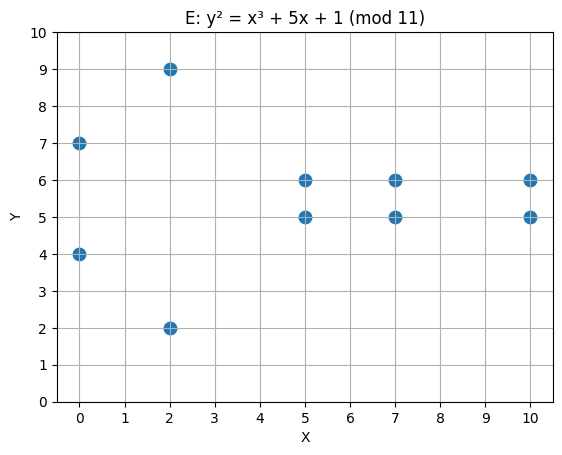
\includegraphics[width=0.5\linewidth]{ell_curve_finite_field.png}
        \caption{Elliptische Kurve über $\mathbb{F}_5$, eigene Darstellung}
        \label{fig:placeholder}
    \end{figure}

    Die Punkte und das Bild wurden mit einem eigenen Python Skript generiert, siehe Anhang.
\end{beispiel}

Um das diskrete Logarithmus für ein Kryptosystem aufbzubauen, müssen wir die Ordnung von einer Gruppe kennen. Dies ist deutlich herausfordernder als das Berechnen des eben gezeigten Beispiels, bei dem extra eine passende Kurve gewählt wurde. Da zuerst überprüft werden muss ob zu einem x Wert der berechnete Wert auch einen quadratischen Rest hat und damit der Punkt exestiert.
\begin{theorem}
Sei $E$ eine elliptische Kurve über einem Körper $K$ und sei $n\in\mathbb N$.
Falls $\operatorname{char}(K)\nmid n$, dann gilt
\[
    E[n]\cong \mathbb Z/n\mathbb Z \oplus \mathbb Z/n\mathbb Z,
\]
wobei
\[
    E[n]=\{P\in E(\overline K)\mid [n]P=\mathcal O\}
\]
die Gruppe der $n$-Torsionspunkte bezeichnet.
\end{theorem}
vgl. \cite{washington08} Washington S.77+79

\begin{proof}
    Der Beweis hierzu ist sehr langwierig und findet sich daher in \cite{washington08} III Abschnitt 3.2.
\end{proof}


\section{Punktzählung}
Im vorangenganen Abschnitt wurde gezeigt wie man bei einfachen Gruppen vorgehen kann um die Ordnung von diesen zu bestimmen. Die Punktzählung für endliche Körper großer Primzahlordnung ist aber sehr unpraktikabel, denn es hat Komplexität \(\O(p^{1+\epsilon}, \epsilon>0)\)(vgl. \cite{schoof95},S. 2020). Daher soll in diesem Abschnitt Ideen entwickelt werden, wie man die Anzahl der Punkte einer Untergruppe von \(E(\mathbb{F}_q)\) berechnen kann.  Dies ist wichtig um später wichtig um passende Bedingungen für eine Kurve für ein Krpyotgraphisches Verfahren zu wählen. Hierfür wird vorallem der Algorithmus von Schoof und die Hasse Schranke benötigt. Der Beweis dieser benötigt eine Vielzahl von Eigenschaften die weit über die Arbeit hinausreichen, daher werden nur einige von ihnen aufgelistet, sodass zumindest eine Skizze des Beweises möglich ist. In \cite{silverman09} S. 138 findet man den ausführlichen Beweise. Dieser Abschnitt basier auf \cite{silverman09}, S.66f.




\subsection{Isogenien und Endmorphismen}
\begin{definition}[Isogenien]
    Seien $E_1$ und $E_2$ elliptische Kurven über
    einem Körper $K$. Eine Isogenie von $E_1$ nach $E_2$
    ist ein Morphismus
    \[
        \phi:E_1\to E_2
        \qquad\text{mit}\qquad
        \phi(\mathcal O_{E_1})=\mathcal O_{E_2}.
    \]
    Die Kurven $E_1$ und $E_2$ heißen isogen, wenn
    eine von null verschiedene Isogenie zwischen
    ihnen existiert, d.h. \(\phi(E_1)\neq\{\mathcal{O}\}\)
\end{definition}
\begin{beispiel}
    Für jedes $m\in\mathbb{Z}$ definiert man die Multiplikationsabbildung
    \[
        [m]: E\to E.
    \]
    Für $m>0$ gilt
    \[
        [m](P)=\underbrace{P+\dots+P}_{m\text{-mal}}.
    \]
    $[m]$ ein Morphismus ist. Für $m=1$ gilt
    $[1]=\operatorname{id}_E$, also ist $[1]$ ein Morphismus. Sei nun
    $[m]$ ein Morphismus. Dann gilt
    \[
        [m+1]=\mu\circ([m],\operatorname{id}_E),
    \]
    wobei $\mu:E\times E\to E$, $(P,Q)\mapsto P+Q$, nach
    \cite[III, Theorem 3.6, S.~64]{silverman09} ein Morphismus ist. Für $m<0$ gilt \[[m](P)=[-m](-P)\]. Da die Negationsabbildung ebenfalls ein Morphismus ist, ist $[m]$ auch für negative $m$ ein Morphismus.
    Schließlich gilt für jedes $m\in\mathbb Z$ die Gleichung
    $[m](\mathcal O)=\mathcal O$. Daher ist $[m]:E\to E$ eine Isogenie.
\end{beispiel}
Aus \cite{silverman09},S.67

\begin{definition}

    Seien \(E_1\) und \(E_2\) elliptische Kurven über einem Körper \(K\), und sei \(\phi:E_1\to E_2\) eine nichtkonstante rationale Abbildung, die über \(K\) definiert ist. Durch Komposition mit \(\phi\) wird eine Einbettung der zugehörigen Funktionenkörper induziert:
    \[
        \phi^*:K(E_2)\to K(E_1),\qquad
        f\mapsto f\circ\phi.
    \]
    Die Abbildung \(\phi\) heißt \textbf{separabel} beziehungsweise inseparabel, wenn die durch \(\phi\) induzierte Körpererweiterung
    \[
        K(E_1)/\phi^*(K(E_2))
    \]
    separabel beziehungsweise inseparabel ist.
    Für eine konstante Abbildung setzt man \(\deg(\phi)=0.\). Ist \(\phi\) nicht konstant, so definiert man den \textbf{Grad} durch
    \[
        \deg(\phi)
        =
        [K(E_1):\phi^*(K(E_2))].
    \]
    Der Grad von \(\phi\) entspricht somit dem Grad der endlichen Körpererweiterung \(K(E_1)/\phi^*(K(E_2))\).

\end{definition}

\begin{lemma}
    \label{lem:deg-isogenien}
    Sei $\phi:E_1\to E_2$ eine von null verschiedene seperable Isogenie zwischen zwei elliptischen Kurven über $K$. Dann gilt
    \[
        \#\ker \phi = \deg \phi,
    \]
    wobei der Kern auf den Punkten über $\overline{K}$ betrachtet wird.
\end{lemma}

\begin{proof}
    Der Beweis hierfür lässt sich in \cite{silverman09}, S.72f.  Theorem III.4.10. (c) finden.
\end{proof}

\subsection{Frobenius-Endomorphismus}
\begin{definition}[Frobenius Abbildung](vgl. \cite{washington08}, S. 98f.)
    \label{def:frobenius}
    Sei $E$ eine elliptische Kurve, gegeben durch eine
    Weierstraßgleichung über $\mathbb F_q$, wobei
    $q=p^r$ eine Primzahlpotenz ist. Die Abbildung
    \[
        \phi_q:E\to E,\qquad
        (x,y)\mapsto(x^q,y^q),\qquad
        \mathcal O\mapsto\mathcal O,
    \]
    heißt Frobenius-Endomorphismus.
\end{definition}

\begin{lemma}
    Sei $E$ eine elliptische Kurve über \(\mathbb{F}_q\). Dann ist $\phi_q$ ein Endomorphismus von $E$ mit dem Grad $q$ und $\phi_q$ ist nicht seperabel.
\end{lemma}
\begin{proof} (vlg. \cite{washington08}, S.52, eventuell etwas ausführlicher)
    Die Abbildung $\phi_q(x,y) = (x^q, y^q)$ ist wohldefiniert, da die Gleichung der elliptischen Kurve Koeffizienten in $\mathbb{F}_q$ besitzt und somit unter der Abbildung $x \mapsto x^q$ invariant ist.

    Da die Gruppenoperation auf $E$ durch rationale Funktionen mit Koeffizienten in $\mathbb{F}_q$ gegeben ist und $\phi_q$ ein Körperhomomorphismus ist, gilt
    \[
        \phi_q(P+Q) = \phi_q(P) + \phi_q(Q)
    \]
    für alle $P,Q \in E(\overline{\mathbb{F}}_q)$.
    Damit ist $\phi_q$ ein Endomorphismus von $E$.

    Der Grad von $\phi_q$ ist $q$.

    Da in Charakteristik $p$ gilt $q = p^r$ und die Ableitung von $x^q$ gleich null ist, ist $\phi_q$ nicht separabel.
\end{proof}

\begin{corollary}
    \label{korr:abbildung-seperabel}
    Sei $E$ eine elliptische Kurve über einem endlichen Körper $\mathbb{F}_q$ mit Charakterstik $p>0$. Dann gilt für den Frobenius-Endomorphismus $\phi:E\to E$ und $m,n\in\mathbb{Z}$, die Abbildung
    \[
        m+n\phi:E\to E
    \]
    ist genau dann seperabel, wenn $p \nmid m$. Daraus folgt die Abbildung $1-\phi$ ist seperabel.
\end{corollary}

\begin{proof}
    Den Beweis findet man in \cite{silverman09}, S.79.
\end{proof}

\begin{corollary}
    \label{kor:gradabbildung}
    Für die elliptische Kurven $E_1$ und $E_2$ ist die Abbildung
    \[
        \deg:\operatorname{Hom}(E_1,E_2)\to\mathbb{Z}, \qquad \phi\mapsto\deg(\phi),
    \]
    eine positivie definite quadratische Form.
\end{corollary}
\begin{proof}
    Ein Beweis findet sich in \cite{silverman09}, S. 85 Korrolar 6.3.
\end{proof}

\subsection{Hasse-Schranke}
\cite{werner02}, S.60--61 und \cite{guneysu24} S.287.
\begin{satz}[Satz von Hasse]
    \label{def:hasse-schranke}
    Sei $E$ eine elliptische Kurve über einem endlichen Kröper $\mathbb{F}_q$. Dann erfüllt die Ordnung von $E(\mathbb{F}_q)$,
    \[|\#E(\mathbb{F}_q)-q-1 |\leq 2\sqrt q\]
\end{satz}
Es ist nun möglich die Gruppenordnung von $E(\mathbb{F})$ rechteinfach abzuschätzen durch
\[
    -2\sqrt{q}+q+1\leq \#E(\mathbb{F})\leq 2\sqrt{q}+q+1.
\]
Dieses Theorem hat nun eine weitrechende Auswirkung auf die Implementierung von elliptischen Kurven, denn Hasses Schranke gibt an, dass wenn wir eine elliptische Kurven mit zum Beispiel $2^{256}$ Elementen benötigen. Benötigen wir eine Primzahl mit in etwa 256 Bit Länge vgl.\cite{guneysu24} S.287.

\begin{definition}[Bilinearform]
    \label{def:biliniearform}
    Sei $V$ ein Vektorraum über einem Körper $K$. Eine Abbildung
    \[
        \langle \cdot,\cdot\rangle:V\times V\to K
    \]
    heißt Bilinearform, falls sie in beiden Argumenten linear ist. Das heißt, für alle $x,y,z\in V$ und $\lambda,\mu\in K$ gilt
    \[
        \langle \lambda x+\mu y,z\rangle
        =
        \lambda\langle x,z\rangle+\mu\langle y,z\rangle
    \]
    sowie
    \[
        \langle x,\lambda y+\mu z\rangle
        =
        \lambda\langle x,y\rangle+\mu\langle x,z\rangle.
    \]
\end{definition}
\begin{satz}[Cauchy-Schwarzsche Ungleichung]
    Für eine Bilinearform auf einem Vektorraum $V$ und $x,y\in V$ gilt
    \[
        \langle x,y\rangle^2\leq \langle x,x\rangle\langle y,y\rangle
    \]
\end{satz}
\begin{proof}
    Ein Beweis findet sich in \cite{poeschel14} S.115.
\end{proof}

\begin{proof}[Hasse]
    Sei $E$ eine elliptische Kurve über \(\mathbb{F}_q\). Außerdem sei \(\phi: E\to E, \quad (x,y)\mapsto (x^q,y^q)\) ein Frobenius Endomorphismus. Für ein $P=(x,y)\in E(\overline{\mathbb{F}}_q$) gilt
    \[
        P\in E(\overline{\mathbb{F}}_q) \Leftrightarrow x,y\in \mathbb{F}_q.
    \]

    Das ist äquivalent zu
    \[
        x^q=x \quad \text{ und } \quad y^q=y.
    \]
    Also gilt
    \[
        \phi(P)=(x^q,y^q)=(x,y)=P.
    \]
    Folglich erhält man
    \[
        P\in E(\mathbb{F}_q), \Leftrightarrow \phi(P)=P.
    \]
    Betrachtet man nun den Endomorphismus
    \[1-\phi:E\to E.\] Für einen Punkt $P\in E(\overline{\mathbb{F}}_q)$ gilt
    \[
        (1-\phi)(P)=\mathcal O
        \Leftrightarrow
        P-\phi(P)=\mathcal O
        \Leftrightarrow
        P=\phi(P).
    \]
    Somit folgt
    \[
        E(\mathbb{F}_q)=\ker(1-\phi).
    \]
    Mit \ref{korr:abbildung-seperabel} folgt $1-\phi$ separabel ist, da p nicht 1 teilt. Nun kann man das Lemma \ref{lem:deg-isogenien} anwenden,
    \[
        \#E(\mathbb{F}_q)
        =\#\ker(1-\phi)
        =\deg(1-\phi).
    \]
    Nach Korollar \ref{kor:gradabbildung} ist die Gradabbildung \(\deg(1-\phi)\) eine positiv definite quadratische Form. Die zugehörige symmetrische Bilinearform ist definiert durch
    \[
        \langle \alpha,\beta\rangle
        =
        \deg(\alpha+\beta)-\deg(\alpha)-\deg(\beta).
    \]
    Es wird nun die Bilinearform verwendet, sodass gilt
    \begin{align*}
        \Leftrightarrow & \langle \alpha,\beta\rangle=\deg(\alpha+\beta)- \deg(\alpha)-\deg(\beta) \\
                        & \deg(\alpha+\beta)= \langle\alpha,\beta\rangle+\deg(\alpha)+\deg(\beta)
    \end{align*}
    Für den gegebenen Fall ist $\alpha=1$ und \(\beta =-\phi\), damit folgt
    \[
        \deg(1-\phi)=\langle 1,-\phi\rangle+\deg(1)+\deg(-\phi)+
    \]
    Es ist \(\deg(1)=1\) und \(\deg(-\phi)=\deg(\phi)=q\) und damit
    \[
        \deg(1-\phi)=\langle 1,-\phi\rangle+1+q
    \]
    mit Biliniearität gilt
    \[
        \deg(1-\phi)=1+q-\langle 1,\phi\rangle.
    \]
    Jetzt fehlt es noch zu zeigen, dass \(|\langle1,\phi\rangle|\leq 2\sqrt{q}\).
    Mit der Cauchy-Schwarz Ungleichung gilt \(|\langle\alpha,\beta\rangle|^2\leq \langle\alpha,\alpha\rangle\langle\beta,\beta\rangle\). Für $\alpha=1$ und \(\beta=\phi\) ergibt sich

    \[
        |
        \langle1,\phi\rangle|^2\leq \langle1,1\rangle\langle\phi,\phi\rangle.
    \]
    Es gilt nach Definition
    \[
        \langle 1,1\rangle = \deg(1+1)-\deg(1) - \deg(1)= 2
    \]
    und
    \[
        \langle\phi,\phi\rangle=\deg(\phi+\phi)-2\deg(\phi)
    \]
    mit \[
        \deg(\phi+\phi)
        =\deg([2]\circ\phi)
        =\deg([2])\deg(\phi)
        =4q
    \]
    folgt
    \[
        \langle\phi,\phi\rangle
        =\deg(\phi+\phi)-2\deg(\phi)
        =4q-2q
        =2q.
    \]
    Nun setzt man noch alles in Cauchy-Schwarz ein, dann folgt
    \[
        |\langle 1,\phi\rangle|^2\leq 2\cdot 2q = 4q
    \]
    und zieht man nun die Wurzel gilt
    \[
        |\langle 1,\phi\rangle|\leq 2\sqrt{q}
    \]
    und damit gilt die gewünschte Aussage.
\end{proof}
\cite{silverman09}, S.138
\cite{silverman06}, S.100






\section{Double-and-Add-Algorithmus}
\label{sec:double-and-add}

Dieser Abschnitt basiert auf \cite{silverman06}, S.30--31 und \cite{buell24}, S.217--218.

Sei $P$ ein Punkt einer additiv geschriebenen Gruppe und
$n \in \mathbb{N}$. Ziel ist es, das skalare Vielfache
\[
    nP = \underbrace{P + P + \dots + P}_{n\text{-mal}}
\]
effizient zu berechnen.

Eine naive Berechnung erfolgt durch sukzessive Addition:
\begin{align*}
    2P & = P + P,      \\
    3P & = 2P + P,     \\
       & \ \vdots      \\
    nP & = (n-1)P + P.
\end{align*}
Hierfür werden insgesamt $n-1$ Gruppenadditionen benötigt. In
Abhängigkeit vom Zahlenwert $n$ liegt die Laufzeit dieser Methode daher in $\mathcal{O}(n)$. Für die Betrachtung der tatsächlichen
Eingabegröße ist jedoch die Anzahl der Bits entscheidend, die zur Darstellung von $n$ benötigt wird. Bezeichnet \(m = \lfloor \log_2(n) \rfloor + 1\) die Bitlänge von $n$, so gilt \( 2^{m-1} \leq n < 2^m \). Der Zahlenwert $n$ wächst somit exponentiell mit seiner Bitlänge
$m$. Daher kann die Laufzeit der naiven Methode äquivalent als \( \mathcal{O}(2^m)\) angegeben werden. Insbesondere bei kryptographischen Verfahren wie dem Diffie-Hellman-Schlüsselaustausch aus
Kapitel 5 ~\ref{sec:diffie-hellman} müssen skalare Vielfache für sehr große Skalare berechnet werden. Die naive Methode ist dafür
nicht praktikabel. Eine wesentlich effizientere Berechnung
ermöglicht der Double-and-Add-Algorithmus.
\cite{guneysu24}, S. 288
\begin{definition}[Double-and-Add-Algorithmus]
    Sei $P$ ein Punkt auf einer elliptischen Kurve $E$ und $n\in \mathbb{N}$. Es soll nun das Vielfache $Q=np$ berechnet werden. Sei \( n = (b_{m-1}b_{m-2}\dots b_0)_2\qquad\text{mit}\qquad b_{m-1}=1\)
    die Binärdarstellung von $n$.Der Double-and-Add-Algorithmus
    verarbeitet die Bits von links nach rechts, beginnend mit dem
    höchstwertigen Bit $b_{m-1}$.
    \begin{enumerate}
        \item Initialisiere $Q = \mathcal{O}$
        \item Führe für $i=m-1,m-2,\dots,0$ die folgenden Schritte aus:
              \begin{enumerate}
                  \item Verdopple den aktuellen Punkt: \( Q = 2Q\)
                  \item Falls $b_i=1$, dann addiere $P$: \(Q=Q+P\)
              \end{enumerate}
    \end{enumerate}
    Nach der Verarbeitung aller Bits gilt $Q=nP$.
\end{definition}
Um die Komplexität zu bestimmen, schreibt man das Skalar $n$ nochmal mit Hilfe der Binärdarstellung
Aus der Binärdarstellung $n=n_0+n_1\cdot 2\cdot 2+n_2\cdot 2^2+\cdots +n_r\cdot 2^r$ mit $n_0,\dots,n_r\in\{0,1\}.$. Daraus folgt für das skalare Vielfache \(nP=n_0P+n_1\cdot2P\cdot 2+n_2\cdot 2^2P+\cdots +N_r\cdot 2^rP\).Der Punkt $2^kP$ wird durch $k$ aufeinanderfolgende Punktverdopplungen berechnet. Da $r=\lfloor\log_2(m)\rfloor$ gilt, benötigt der Double-and-Add-Algorithmus genau $\lfloor\log_2(m)\rfloor$ Verdopplungen. Bei annähernd gleichverteilten Bits kommen im Mittel etwa \(\frac{1}{2}\lfloor\log_2(m)\rfloor\) Punktadditionen hinzu. Die Laufzeit liegt somit in
$\mathcal{O}(\log m)$.
\begin{beispiel}
    Es soll das skalare Vielfache $46P$ berechnet werden. Zunächst
    wird der Skalar in Binärdarstellung überführt \( 46=(101110)_2\).
    Die Verarbeitung beginnt beim höchstwertigen Bit (\emph{most significant bit}, MSB). Da dieses stets gleich $1$ ist, wird der Startwert $Q=P$ gesetzt. Anschließend werden die
    verbleibenden Bits von links nach rechts verarbeitet.
    \begin{table}[htbp]
        \centering
        \begin{tabular}{c l l}
            \hline
            \textbf{Bit} & \textbf{Operation}       & \textbf{Zwischenergebnis} \\
            \hline
            $1$          & Initialisierung          & $Q=P$                     \\
            $0$          & Verdopplung              & $Q=2P$                    \\
            $1$          & Verdopplung und Addition & $Q=5P$                    \\
            $1$          & Verdopplung und Addition & $Q=11P$                   \\
            $1$          & Verdopplung und Addition & $Q=23P$                   \\
            $0$          & Verdopplung              & $Q=46P$                   \\
            \hline
        \end{tabular}
        \caption{Berechnung von $46P$ mit dem Double-and-Add-Algorithmus}
        \label{tab:double-and-add-26}
    \end{table}

    Für die Berechnung von $46P$ werden somit fünf Verdopplungen und
    drei zusätzliche Additionen benötigt. Insgesamt sind dies sechs
    Gruppenoperationen. Die naive Methode würde dagegen
    $46-1=45$ Additionen erfordern.
\end{beispiel}



\subsection{Baby steps and giant steps}
\cite{schoof95}, S.220 Komplexität ist \(\O(p^{1/4+\epsilon}), \epsilon>0\). Praktisch für großere Primzahlen, aber unpraktisch für Zahlen größer 20 Dezimalstellen

Es wird Hasse benötigt.
\subsection{Schofs Algorithm}


\chapter{Elliptische Kurven Kryptographie}
Nun wie wird aus abstrakter Mathematik ein kryptographisches Verfahren. In Kapitel 2 wurde schon Public-Key Kryptographie und das DL Problem betrachtet. Das selbe Prinzip soll nun genutzt werden, um ein kryptographisches Verfahren basierenden auf elliptischen Kurven zu implementieren. 
\label{sec:kryptographie}
\section{Diffie-Hellman}
\label{sec:diffie-hellman}
basiert auf \cite{washington08}, S.170-172
Wir betrachten eine möglichkeit einen geheimen Schlüssel zu etablieren nach Diffie und Hellman. Außerdem verwendet \cite{fuß25}, S. 195
\begin{enumerate}
    \item Alice und Bob einigen sich auf eine elliptische Kurve $E:y^2=x^3+Ax+B\mod p$ über einem endlichen Körper $\mathbb{F}_p$, sodass das diskrete Logarithmusproblem in $E(\mathbb{F}_p)$ schwer zu lösen ist.
    \item Alice wählt ein geheimes $a$, das ein Integer sein soll, berechne $P_a=aP$ und schickt $P_a$ zu Bob.
    \item BoB wählt einen geheimen Integer b, er berechnet $P_b=bP$ und schickt Alice $P_b$.
    \item Alice berechnet $aP_b=abP$
    \item Bob berechnet $bP_a=baP$
    \item Alice und Bob benutzen eine öffentliche Methode um einen Schlüssel von $abP$ zu extrahieren. Zum Beispiel könnten sie die letzten 256 bits der x-Koordinate von $abP$ als Schlüssel verwenden oder sie könnten eine Hash-Funktion auf der x-Koordinate definieren.
\end{enumerate}
Die einzige Information die ein Außenstehender sieht, wäre die Kurve $E$, den Körper $F_q$ und die Punkte $P, aP,bP$. Daher muss sie das \textbf{Diffie-Hellman Problem} lösen.

\begin{definition}[Diffie-Hellman Problem]
    Sei $P,aP,bP\in E(\mathbb{F}_q)$ gegeben berechne
    \[
        abP.
    \]
\end{definition}


\begin{beispiel}
    Wir betrachten die elliptische Kurve
    \[
        E\colon y^2 \equiv x^3+2x+2 \pmod{17}
    \]
    über dem Primkörper \(\mathbb F_{17}\). Durch explizite Bestimmung der Punkte erhält man
    \[
        \#E(\mathbb F_{17})=19.
    \]
    Da die Gruppenordnung \(19\) eine Primzahl ist, erzeugt jeder
    Punkt aus \(E(\mathbb F_{17})\setminus\{\mathcal O\}\) die gesamte
    Gruppe. Im Folgenden wird der Generator
    \[
        P=(0,6)
    \]
    gewählt. Die Berechnung der Ordnung, des Generators und alle weiteren Punktberechnungen wurde mit Hilfe des im Anhang~\ref{app:pythonprogramm} angegebene und selbstentickwelten Python-Programm durchgeführt.
    Alice wählt die geheime Zahl $a=2$ und berechnet den öffentlichen Schlüssel $A=aP=2P=(9,1)$, anschließend schickt Alice Bob $P_a$. Bob wählt $b=5$ und berechnet $B=bP=5P=(10,11)$, anschließend schickt Bob Alice $P_b$. Alice berechnet nun ihren gemeinsamen Schlüssel $S_A=aP_b=2\cdot(10,11)=(16,4)$, genauso wie Bob $S_B=bP_a=5\cdot(9,1)=(16,4)$.  Im Beispiel gilt konkret
    \[
        2B=2\cdot5P=10P=5\cdot2P=5A=(16,4).
    \]
    Öffentlich bekannt sind die Kurve \(E\), der Körper
    \(\mathbb F_{17}\), der Basispunkt \(P\) sowie die Punkte
    \(A=aP\) und \(B=bP\). Die Zahlen \(a\) und \(b\) sowie der
    gemeinsame Punkt \(S=abP\) werden dagegen nicht übertragen.

    Ein Angreifer müsste dann wie beschrieben, dass Diffie-Hellman-Problem lösen und \(abP\) finden. Eine Möglichkeit wäre \(a\) aus \(aP\) oder \(b\) aus \(bP\) mit dem diskreten Logarithmus Problem zu lösen. Anschließend könnte der Angreifer den gemeinsamen Punkt
    durch
    \[
        aB=a(bP)=abP
    \].Bei der hier betrachteten Gruppe mit nur \(19\) Elementen kann der
    diskrete Logarithmus durch einfaches Berechnen der Vielfachen
    \[
        P,2P,3P,\ldots
    \]
    gefunden werden. Bei kryptographisch verwendeten Kurven arbeitet man
    dagegen in einer Untergruppe von sehr großer Primzahlordnung. Eine
    vollständige Aufzählung der Vielfachen von \(P\) ist dort praktisch
    nicht durchführbar.
\end{beispiel}

Um eine sichere Konfiguration für Diffie-Hellman zu erhalten muss $p$ relativ groß ($p>2^{160})$ und daher muss man eine große Anzahl von Vielfachen von einem Punkt $P$ berechnen
\[
    mP = P +P +P+\dots P\in E(\mathbb{F}_p).
\]
Wenn man
\cite{silverman06}, S. 30


Diffie-Hellman in dieser Form führt nur dazu, dass ein gemeinsamer Schlüssel ausgetauscht wird, es gibt noch keine Beschreibung wie genau die Verschlüsslung und Entschlüsslung funktioniert. Dazu kann man zum Beispiel das ElGamal Public Key Verfahren verwenden. 
Alice möchte Bob eine Nachricht senden. Dafür muss Bob aber seinen öffentlichen Schlüssel etablieren. Dafür wählt er eine elliptische Kurve $E$ über einem endlichen Körper $\mathbb{F}_q$, so dass das DL Problem schwer zu lösen ist auf $E\mathbb{F}_q$ (wie genau diese Bedingungen sein muss wird in Abschnitt \ref{sicherheitsbetrachtung} betrachtet). Außerdem wählt er auch einen Punkt $P$ auf $E$. Er wählt wieder einen geheimes $b\in\mathbb{Z}$ und berechnet $B=bP$. Die elliptische Kurve $E$, der endliche Körper $\mathbb{F}_q$ und die Punkte $P$ und $B$ macht er öffentlicht und dienen ihm als öffentliche Schlüssel. Wenn Alice Bob eine Nachricht schicken möchte geht sie wie folgt vor
\begin{enumerate}
    \item Alice lädt Bobs öffentlichen Schlüssel runter
    \item Sie schreibt ihre Nachricht als ein Punkt $M\in E(\mathbb{F}_q)$
    \item Nun wählt Alice einen geheimen Schlüssel $k$ und berechnet $M_1=kP$
    \item Anschließend berechnet Alice $M_2=M+kB$
    \item Nun sendet Alice $M_1,M_2$ an Bob
\end{enumerate}

Bob entschlüsselt die Nachricht indem er \(M=M_2-bM_1\) berechnet. Das funktioniert da Bob $b$ kennt und daher 
\[
    M_2-bM_1=(M+kB)-s(kP)= M+k(bP)-bkP=M
\]
berechnen kann. Eine dritte Person Eve die die Nachrichten $M_1$ und $M_2$ abfängt, kann nur durch Lösen des DL-Problems $b$ aus den öffentlichen Informationen $P$ und $B$ berechnen. Wenn sie $b$ nicht errechnen, kann exestiert kein Weg um die Nachricht $M$ zu entschlüsseln.
\begin{bemerkung}
    In der Regel wird mit asymmetrischen Verfahren nur ein symmetrischer Schlüssel ausgetauscht und daher handelt es sich meist bei der Nachricht um einen Punkt auf der Kurve der als Geheimnis dient zum Beispiel wird die x-Koordinate des gemeinsamen Schlüssels verwendet und mit einer Hashfunktion verschlüsselt und dann als symmetrischer Schlüssel verwendet (vgl. \cite{guneysu24}, S.291). Wenn tatsächlich eine richtige Nachricht wie zum Beispiel "Hallo" geschickt werden soll, dann muss diese zuerst in ihre Bitdarstellung überführt werden, zum Beispiel mit Hilfe von ASCII und anschließend dann mit einer Abbildung auf einen Punkt auf der Kurve abgebildet werden.
\end{bemerkung}

\begin{bemerkung}
    Wenn Alice das selbe $k$ zweimal verwendet, ist $M_1'=kP=M_1$. Eve kann das Wissen nutzen, um $M$ zu berechnen indem sie $M_2'-M_2= M'-bM_1'-(M-bM_1)=M'-M$ berechnet. Wenn Eve nun Wissen über $M$ erhält, kann sie dadurch auch automatisch $M'$ berechnen und alle weiteren Nachrichten die anschließend mit $k$ verschlüsselt werden.
\end{bemerkung}


\cite{washington08}, S. 174-176
\begin{definition}[ElGamal Verschlüsslung]

    Es exestiert nun zum erzeugten Schlüssel $(ab)\cdot G$ eine Funktion
    \[
    F: E \to E, P\mapsto P+(ab)\cdot G
    \]
    Es gibt dann eine Verschlüsslungsfunktion
    \[
    P\mapsto (B,Q)= (b\cdot G,P+b\cdot A)
    \]
    und eine Entschlüsslungsfunktion
    \[
    (B,Q)\mapsto Q-a\cdot B=Q-(ab)\cdot G=Q-b\cdot A=P
    \]
\end{definition}
Exklusives Geheimnis von Alice ist einzig die Zahl a. Bobs Geheimnis ist nur die Zahl b. Beide Zahlen können aus den Punkten $A=a\cdot G$ und $B=b\cdot G$ nicht zurückgerechnet werden.
\begin{bemerkung}
    Wie beim klassischen Elgamal-Verfahren muss Bob jedes mal eine neue Zahl $b$ auswählen. Denn ansonsten kann aus dem Geheimtext \(b\cdot G, P+b\cdot A\) mit Klartext $P$, der Kurvenpunkt $b\cdot A$ bestimmt werden. Dadurch können alle andere Punkte die mit $b$ verschlüsselt wurden entschlüsselt werden.
\end{bemerkung}
\section{ECDSA}

\section{Eventuell noch ECIES \cite{washington08},S.180ff.}
\section{Warum eliptische Kurven verwenden?}
Der beste Algorithm um ECDLP zu lösen ist exponential, darum werden Elliptische Kurven Gruppen verwendet. (An Introduction to the Theory of Elliptic Curves, S.6)
Genauer der beste Algorithmus um ECDLP zu lösen über $\mathbb{F}_p$ braucht $O(\sqrt p)$ Zeit.


Ephemeral-Diffie-Hellman-Key-Agreement mit elliptischen
Kurven

ECDSA


\section{Sicherheitbetrachtung und Wahl von sinnvollen Bedingugen}
\label{sicherheitsbetrachtung}
\textbf{Warum elliptische Kurven?}
Praktisch stellt sich das RSA-Verfahren erst ab einer Schlüsselänge von 3000 Bit als sicher heraus. Entsprechend aufwendig gestaltet sich dort das Ver- und
Entschlüsseln. Um das Verschlüsseln effizient zu gestalten, kann ein kleiner Exponent e gewählt werden. Elliptische Kurven haben sich in der modernen Kryptographie etabliert, weil sie bei vergleichbarem Sicherheitsniveau deutlich kürzere Schlüssellängen erfordern als klassische Verfahren wie RSA.     So bietet ein RSA-Schlüssel mit 4096 Bit ein Sicherheitsniveau, das mit Verfahren auf Basis elliptischer Kurven bereits mit einer Schlüssellänge von etwa 313 Bit erreicht werden kann (vgl. \cite{washington08}, S. 169). Dies führt zu geringerem Speicherbedarf, ermöglicht kompaktere Hardware und reduziert den Energieverbrauch.
Elliptische Kurven bieten nun eine Möglichkeit um, wie wir in den folgenden Kapiteln sehen werden, ein schwer zu lösendes diskretes Logarithmus Problem zu stellen.
Faktorisierung großer Zahlen (Computeralgebra Kapitel 5, ab S.167)
\textbf{Weil-Pairing?}


\begin{itemize}
    \item Punktzählung
    \item Baby Step Giant Step
    \item Pohlig-Hellman zeigt, dass man Untergruppen großer Primzahlordnung braucht
    \item MOV 
\end{itemize}
\section{Performancesteigerung und Vergleich von ECC zu anderen Verfahren}

Performance wäre zu finden bei \cite{fuß25}, S.201

\cite{fuß25}, S.199-200

\begin{figure}[htbp]
    \centering
    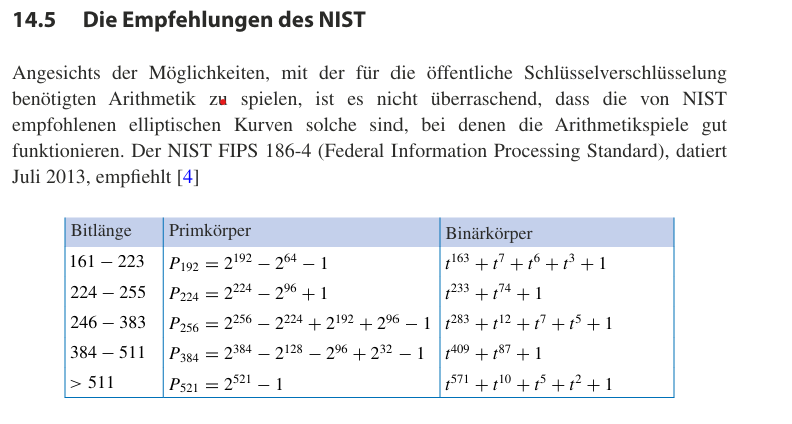
\includegraphics[width=\linewidth]{empfehlung_der_nist.png}
    \caption{Empfehlungen des NIST, entnommen aus \cite[S.~219]{buell24}.}
    \label{fig:nist-empfehlungen}
\end{figure}

\section{Angriffe auf ECC}
In Kapitel 2 \ref{baby-step-giant-step} wurde der Baby Step Giant Step Algorithmus verwendet nun soll dieser nochmal an einem Beispiel für elliptische Kurven aufgegriffen werden.
\begin{beispiel}
    Es wird erneut das Beispiel aus Kapitel 4 aufgegriffen, aber es wird angenommen, dass die Gruppenordnung unbekannt sei. Sei $G=E(\mathbb{F}_{17})$, wobei $E$ gegeben ist durch $y^2=x^3+2x+2$. Sei $P=(0,6)$ und $Q=(3, 16)=kP$. nach dem Satz von Hasse \ref{def:hasse-schranke} kann eine obere Schranke ausgerechnet werden
    \[ 
    |\#E(\mathbb{F}_{17})-17-1 |\leq 2\sqrt 17
    \],
    also die Ordnung maximal 26. Daher sei $m=\lceil \sqrt{26}\rceil=6$. Die Punkte $iP$ für $1\leq i< 6$ sind
    \[
    (0, 6), (9, 1), (6, 3), (7, 6), (10, 11)
    \]
    Für die linke Seite wird dann $Q-jmP$ berechnet für $j=0,1,2,3,4$
    \[
    (3,16),(13, 10),(0, 6),(10, 6),(5,16),(9,1).
    \]
    Es wird bei $j=2$ beendet, da der Punkt mit $1P$ übereinstimmt. Nun kann k einfach nachgerechnet werden, 
    \[
    (30,40)=kP=(1+2\cdot6)P= 13P
    \]
    und damit erhalten wir $k=13$ als das gesuchte Ergebnis.
    Alles wurde mit Hilfe von \ref{app:pythonprogramm}, die Konsolenausgabe ist in \ref{fig:python-2}.
\end{beispiel}
Nun wird das Pohlig Hellmann Verfahren aus Kapitel 2 \ref{pohlig-hellman} ebenefalls für elliptische Kurven aufgegriffen.
\begin{beispiel}
    Sei $G=E(\mathbb{F}_{599})$ für die elliptische Kurve
    $E\colon y^2=x^3+1$. Gegeben seien die Punkte
    $P=(60,19)$ und $Q=(277,239)$. Das Python-Programm
    liefert $|G|=\operatorname{ord}(P)=600$. Gesucht ist
    ein $k\in\{0,\dots,599\}$ mit $Q=kP$.
    Wegen $600=2^3\cdot3\cdot5^2$ bestimmen wir wie in
    Kapitel~2 zunächst $k$ modulo $8$, $3$ und $25$.
    Alle Koordinatenrechnungen erfolgen modulo $599$.

    \smallskip
    \noindent\textbf{Bestimmung von $k\bmod 8$.}
    Wir schreiben $k\equiv z_0+2z_1+4z_2\pmod 8$
    mit $z_i\in\{0,1\}$. Der Punkt
    $R=\frac{600}{2}P=300P=(598,0)$ hat die Ordnung $2$.
    Die Berechnung ergibt $300Q=e_G=0R$, also $z_0=0$.
    Die weiteren Ziffern ergeben sich aus
    \[
    \begin{aligned}
        Q_1&=\frac{600}{2^2}(Q-z_0P)
             =150Q=(598,0)=R,\\
        Q_2&=\frac{600}{2^3}(Q-(z_0+2z_1)P)
             =75(Q-2P)=75(35,243)=e_G.
    \end{aligned}
    \]
    Somit sind $z_1=1$ und $z_2=0$, weshalb
    $k\equiv 0+2\cdot1+4\cdot0=2\pmod 8$ gilt.

    \smallskip
    \noindent\textbf{Bestimmung von $k\bmod 3$.}
    Hier ist $R=\frac{600}{3}P=200P=(0,1)$.
    Aus $200Q=(0,598)=2R$ folgt unmittelbar
    $k\equiv2\pmod 3$.

    \smallskip
    \noindent\textbf{Bestimmung von $k\bmod 25$.}
    Wir schreiben $k\equiv z_0+5z_1\pmod{25}$
    mit $z_0,z_1\in\{0,\dots,4\}$ und setzen
    $R=\frac{600}{5}P=120P=(84,179)$.
    Aus $120Q=(84,179)=R$ folgt $z_0=1$.
    Anschließend berechnen wir
    \[
        Q_1=\frac{600}{5^2}(Q-P)
            =24(130,129)=(491,465)=3R.
    \]
    Daher ist $z_1=3$ und damit
    $k\equiv1+5\cdot3=16\pmod{25}$.

    \smallskip
    \noindent\textbf{Zusammensetzen der Ergebnisse.}
    Aus $k\equiv2\pmod 8$ und $k\equiv2\pmod 3$
    folgt $k\equiv2\pmod{24}$.
    Mit $k=2+24t$ ergibt die verbleibende Kongruenz
    \[
        2+24t\equiv16\pmod{25}
        \quad\Longleftrightarrow\quad
        t\equiv11\pmod{25}.
    \]
    Somit gilt $k\equiv266\pmod{600}$.
    Der gesuchte diskrete Logarithmus ist also $k=266$.
\end{beispiel}

\subsection{MOV-Algorithmus}
\cite{washington08} S. 156--157
\begin{lemma}
    Sei $E$ eine elliptische Kurve über dem Körper $\mathbb{F}_q$ mit
    \[
        \operatorname{Spur}(\phi_q)
        = q+1-\#E(\mathbb{F}_q)=0.
    \]
    Sei $n\in\mathbb{Z}_{>0}$. Existiert ein Punkt
    $P\in E(\mathbb{F}_q)$ der Ordnung $n$, so gilt
    \[
        E[n]\subseteq E(\mathbb{F}_{q^2}).
    \]
\end{lemma}

Dadurch kann das diskrete Logarithmusproblem auf einer supersingulären elliptischen Kurve mit $\operatorname{Spur}(\phi_q)=0$ auf ein diskretes Logarithmusproblem in der multiplikativen Gruppe $\mathbb{F}_{q^2}^{\times}$ reduziert werden. Da hierfür lediglich eine
Körpererweiterung vom Grad $2$ benötigt wird, können effizientere Verfahren zur Berechnung diskreter Logarithmen in endlichen Körpern
angewendet werden.

Auch für supersinguläre Kurven mit $\operatorname{Spur}(\phi_q)\neq 0$ ist eine solche Reduktion möglich. Dabei kann ein rweiterungsgrad $m\in\{3,4,6\}$ erforderlich sein. Diese Erweiterungsgrade sind weiterhin klein und ermöglichen daher eine Beschleunigung der Berechnung des diskreten Logarithmus.
\chapter{Implementierung und Angriffe}
\section{Design}
\section{Punktaddition}
\section{Skalarmultiplikation}
\section{Implemeneiterun von ECDH}

Für Implementierung im Computer sind verschiedene Koordinaten System unterschiedlich schnell, da die Operationen auf diesen von Punkte unterschiedlich schnell sein können. Daher Rosen Kapitel 2.6, S.42 für mehr Infos anschauen.
\section{Verlgeich zu klassichem Diffie-Hellman}

\section{Angriffe}
General number field sieve
\section{Pohling Helman Verfahren}
\section{MOV Algorithmus}
\chapter{Quantencomputer}
Modern Crypography (S.397)
Laufzeit, Schlüsselgrößen, Sicherheit

Alles schön Visualisieren

\printbibliography

\section{Anhang}
\label{app:pythonprogramm}

\end{document}
